% Start appendix section
\newpage
\appendix

% Main APPENDICES heading (only appears once)
\begin{center}
	% Remove \thispagestyle{plain} to maintain consistent page numbering
	{\large\bf APPENDICES}\\[12pt]
\end{center}
\addcontentsline{toc}{chapter}{APPENDICES}

% Appendix A content
\begin{center}
	% Remove \thispagestyle{plain} to maintain consistent page numbering
	{\bf APPENDIX A}\\[36pt]
\end{center}
\addcontentsline{toc}{section}{APPENDIX A}

\begin{center}
	GANTT CHART
	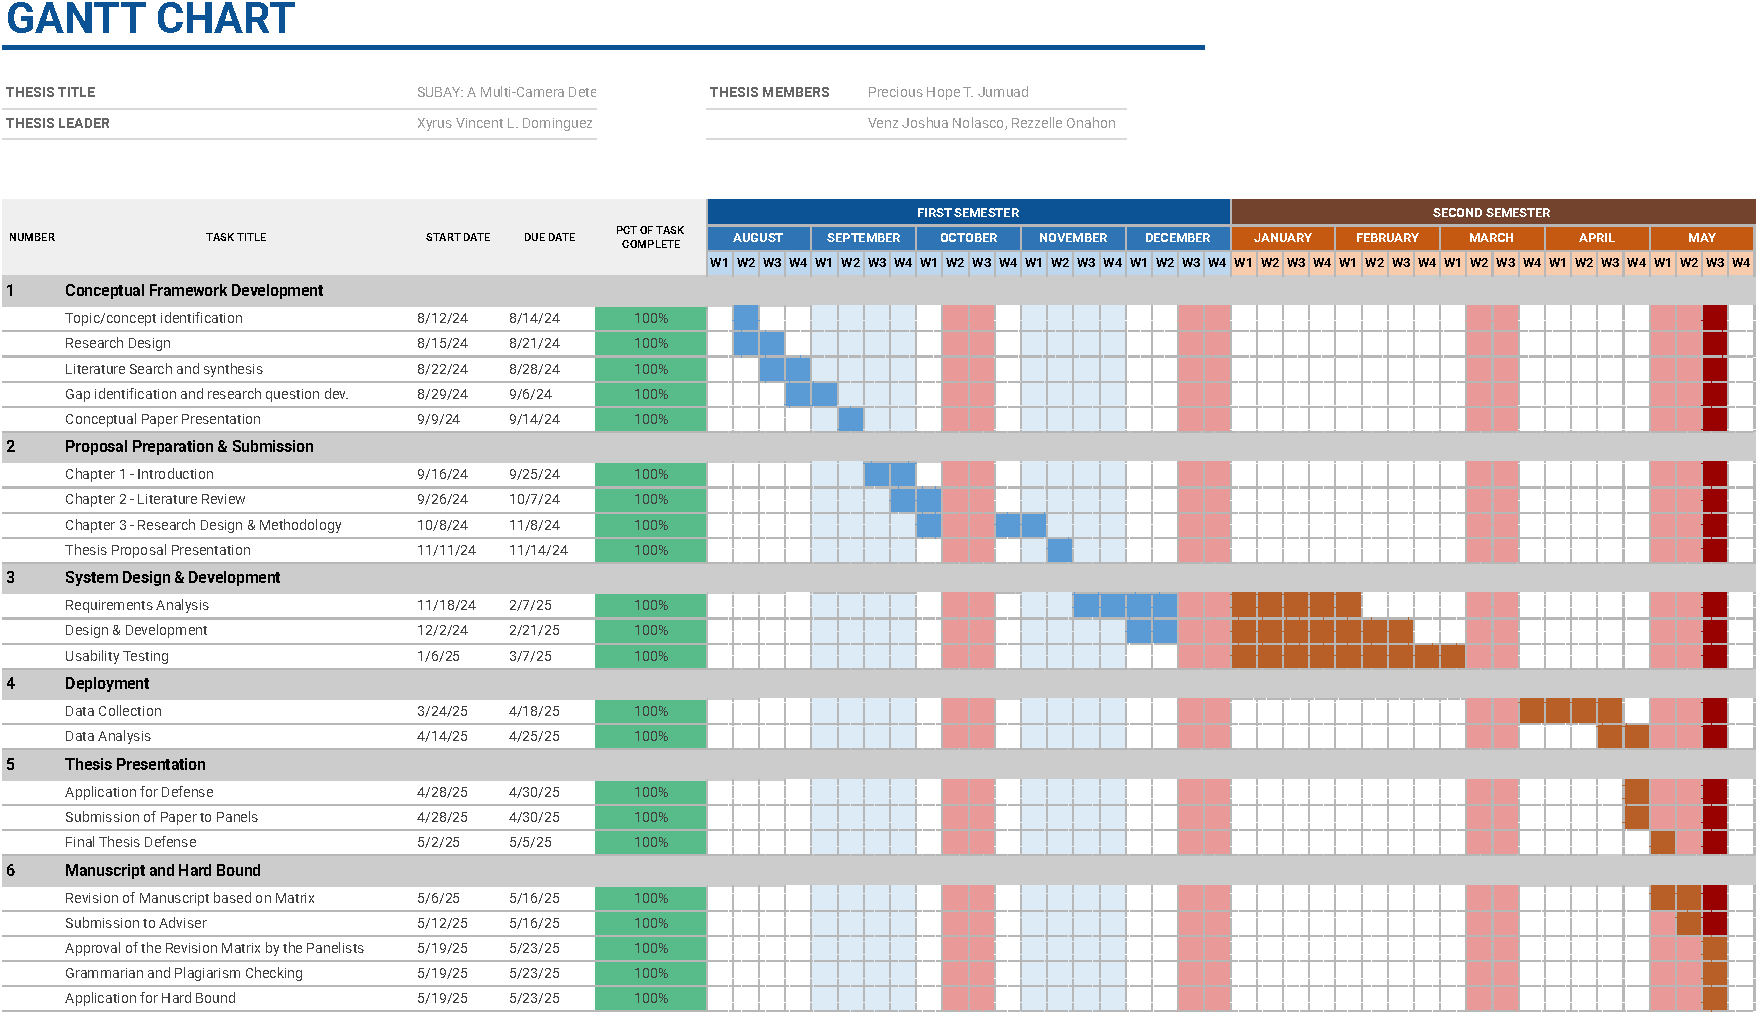
\includegraphics[width=1\textwidth]{app/AA.pdf}
\end{center}

\clearpage

\begin{center}
	% Remove \thispagestyle{plain} to maintain consistent page numbering
	{\bf APPENDIX B}\\[18pt]
\end{center}
\addcontentsline{toc}{section}{APPENDIX B}

\begin{center}
	LETTER OF CONSENT
\end{center}

\vspace{8pt}

% Set smaller font size for the entire letter
\footnotesize

\noindent April 8, 2025

\vspace{8pt}

\noindent \textbf{BABYLYN DIMALILAY}\\
Owner, FashionLane Gift Shop\\
Market City, Agora, Lapasan, Cagayan de Oro City

\vspace{8pt}

\noindent Dear Ms. Dimalilay:

\vspace{6pt}

\noindent Warm greetings!

\vspace{4pt}

\noindent The undersigned are Bachelor of Science in Computer Engineering students at the University of Science and Technology of Southern Philippines. We are researching and discovering the requirements of users, customers, and other stakeholders for a thesis to develop a multi-camera person detection system for tracking and monitoring customer movement in your store. The information that will be gathered will be very beneficial in the design and implementation of the thesis.

\vspace{4pt}

\noindent In view thereof, we formally request your permission to conduct a document review, observation, and interview in your enterprise. Rest assured that the information collected from you will only be used for specific purposes within the framework of the project. All information will be treated with the utmost confidentiality in compliance with the Data Privacy Act of 2012 (R.A. 10173). Specifically, we commit to the following:

\vspace{4pt}

\begin{enumerate}
	\setlength{\itemsep}{0pt}
	\setlength{\parskip}{0pt}
	\item Data will be used solely for academic purposes.
	\item Information collected will be anonymized to ensure individual privacy.
	\item Data storage will comply with industry standards for security, and access will be restricted to authorized researchers only.
	\item All records will be permanently deleted upon the study's conclusion.
\end{enumerate}

\vspace{4pt}

\noindent We greatly appreciate your support and collaboration in this endeavor. Please do not hesitate to contact us at +639608374144 for any concerns or clarifications. We hope you approve this request.

\vspace{8pt}

\noindent Sincerely yours,

\vspace{16pt}

\begin{minipage}[t]{0.48\textwidth}
	\noindent\underline{\textbf{XYRUS VINCENT L. DOMINGUEZ}}\\
	Research Leader
\end{minipage}%
\hfill
\begin{minipage}[t]{0.48\textwidth}
	\noindent\underline{\textbf{PRECIOUS HOPE T. JUMUAD}}\\
	Research Member
\end{minipage}

\vspace{8pt}

\begin{minipage}[t]{0.48\textwidth}
	\noindent\underline{\textbf{VENZ JOSHUA NOLASCO}}\\
	Research Member
\end{minipage}%
\hfill
\begin{minipage}[t]{0.48\textwidth}
	\noindent \underline{\textbf{REZZELLE T. ONAHON}}\\
	Research Member
\end{minipage}

\vspace{16pt}

\noindent Noted by:

\vspace{8pt}

\noindent \underline{\textbf{ENGR. JODIE REY D. FERNANDEZ}}\\
Thesis Adviser/Faculty, Computer Engineering Department

\clearpage

\begin{center}
	% Remove \thispagestyle{plain} to maintain consistent page numbering
	{\bf APPENDIX C}\\[24pt]
\end{center}
\addcontentsline{toc}{section}{APPENDIX C}

\begin{center}
	OBSERVATION CONDUCTED ON ZONE/AISLES
\end{center}

\setlength{\LTleft}{0pt}
\setlength{\LTright}{0pt}
\begin{center}
	\begin{longtable}{|>{\centering\arraybackslash}m{0.48\textwidth}|>{\centering\arraybackslash}m{0.48\textwidth}|}
		\hline
		\textbf{Zone A / Aisle 1} & \textbf{Zone B / Aisle 2} \\
		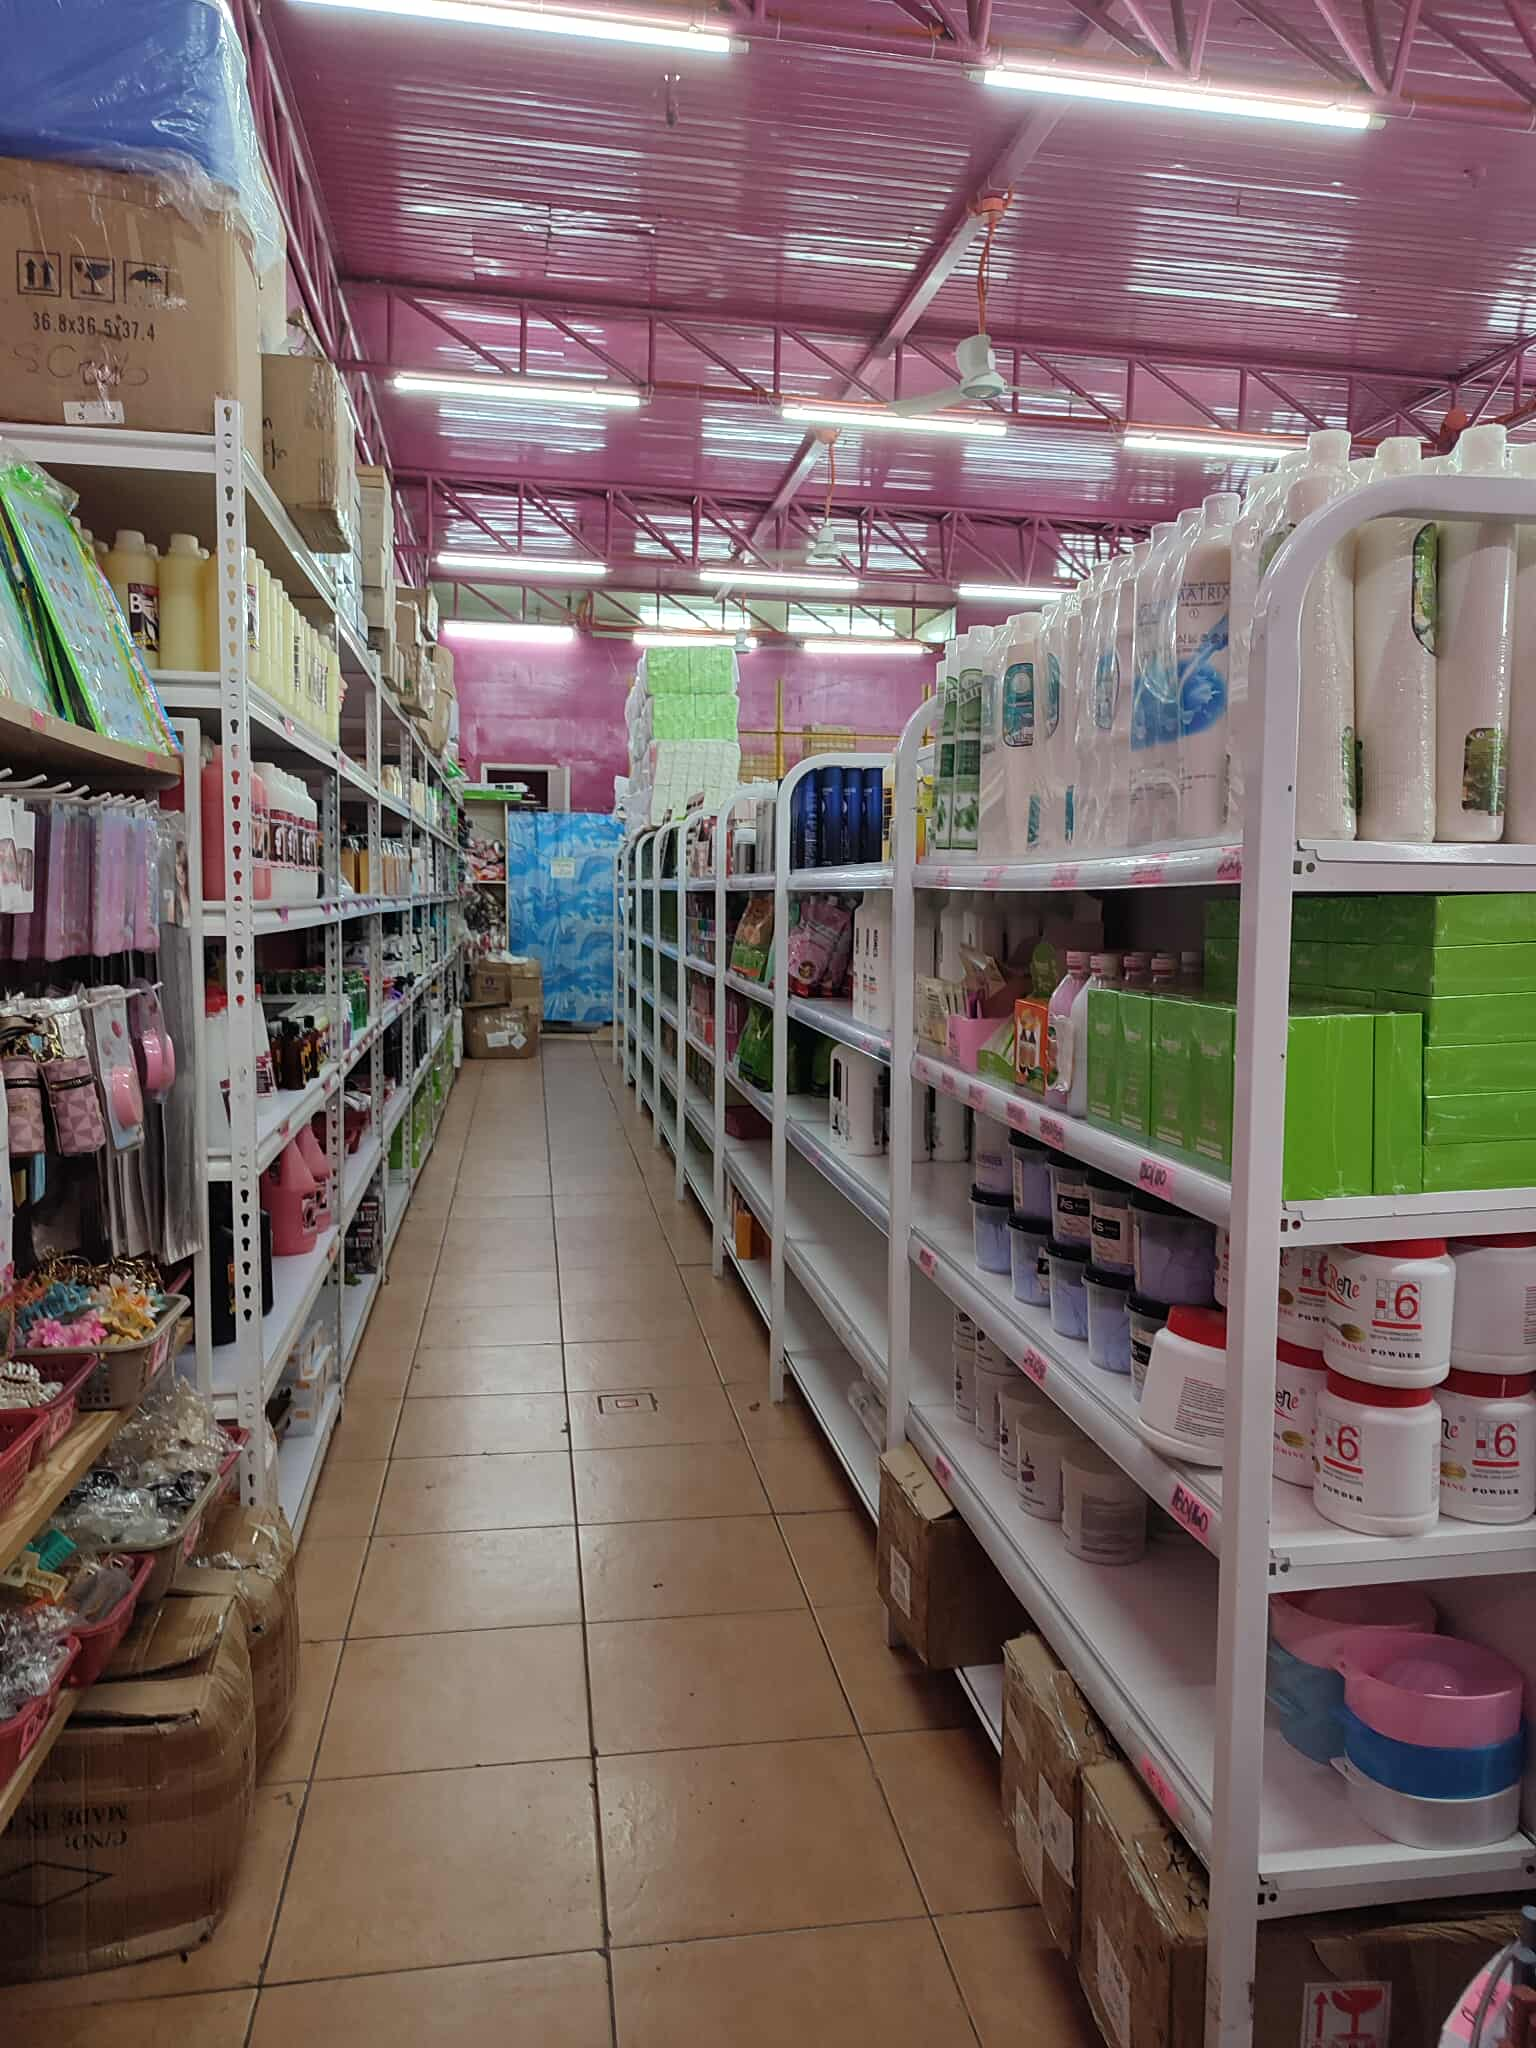
\includegraphics[width=0.30\textwidth]{appendices/zone1} & 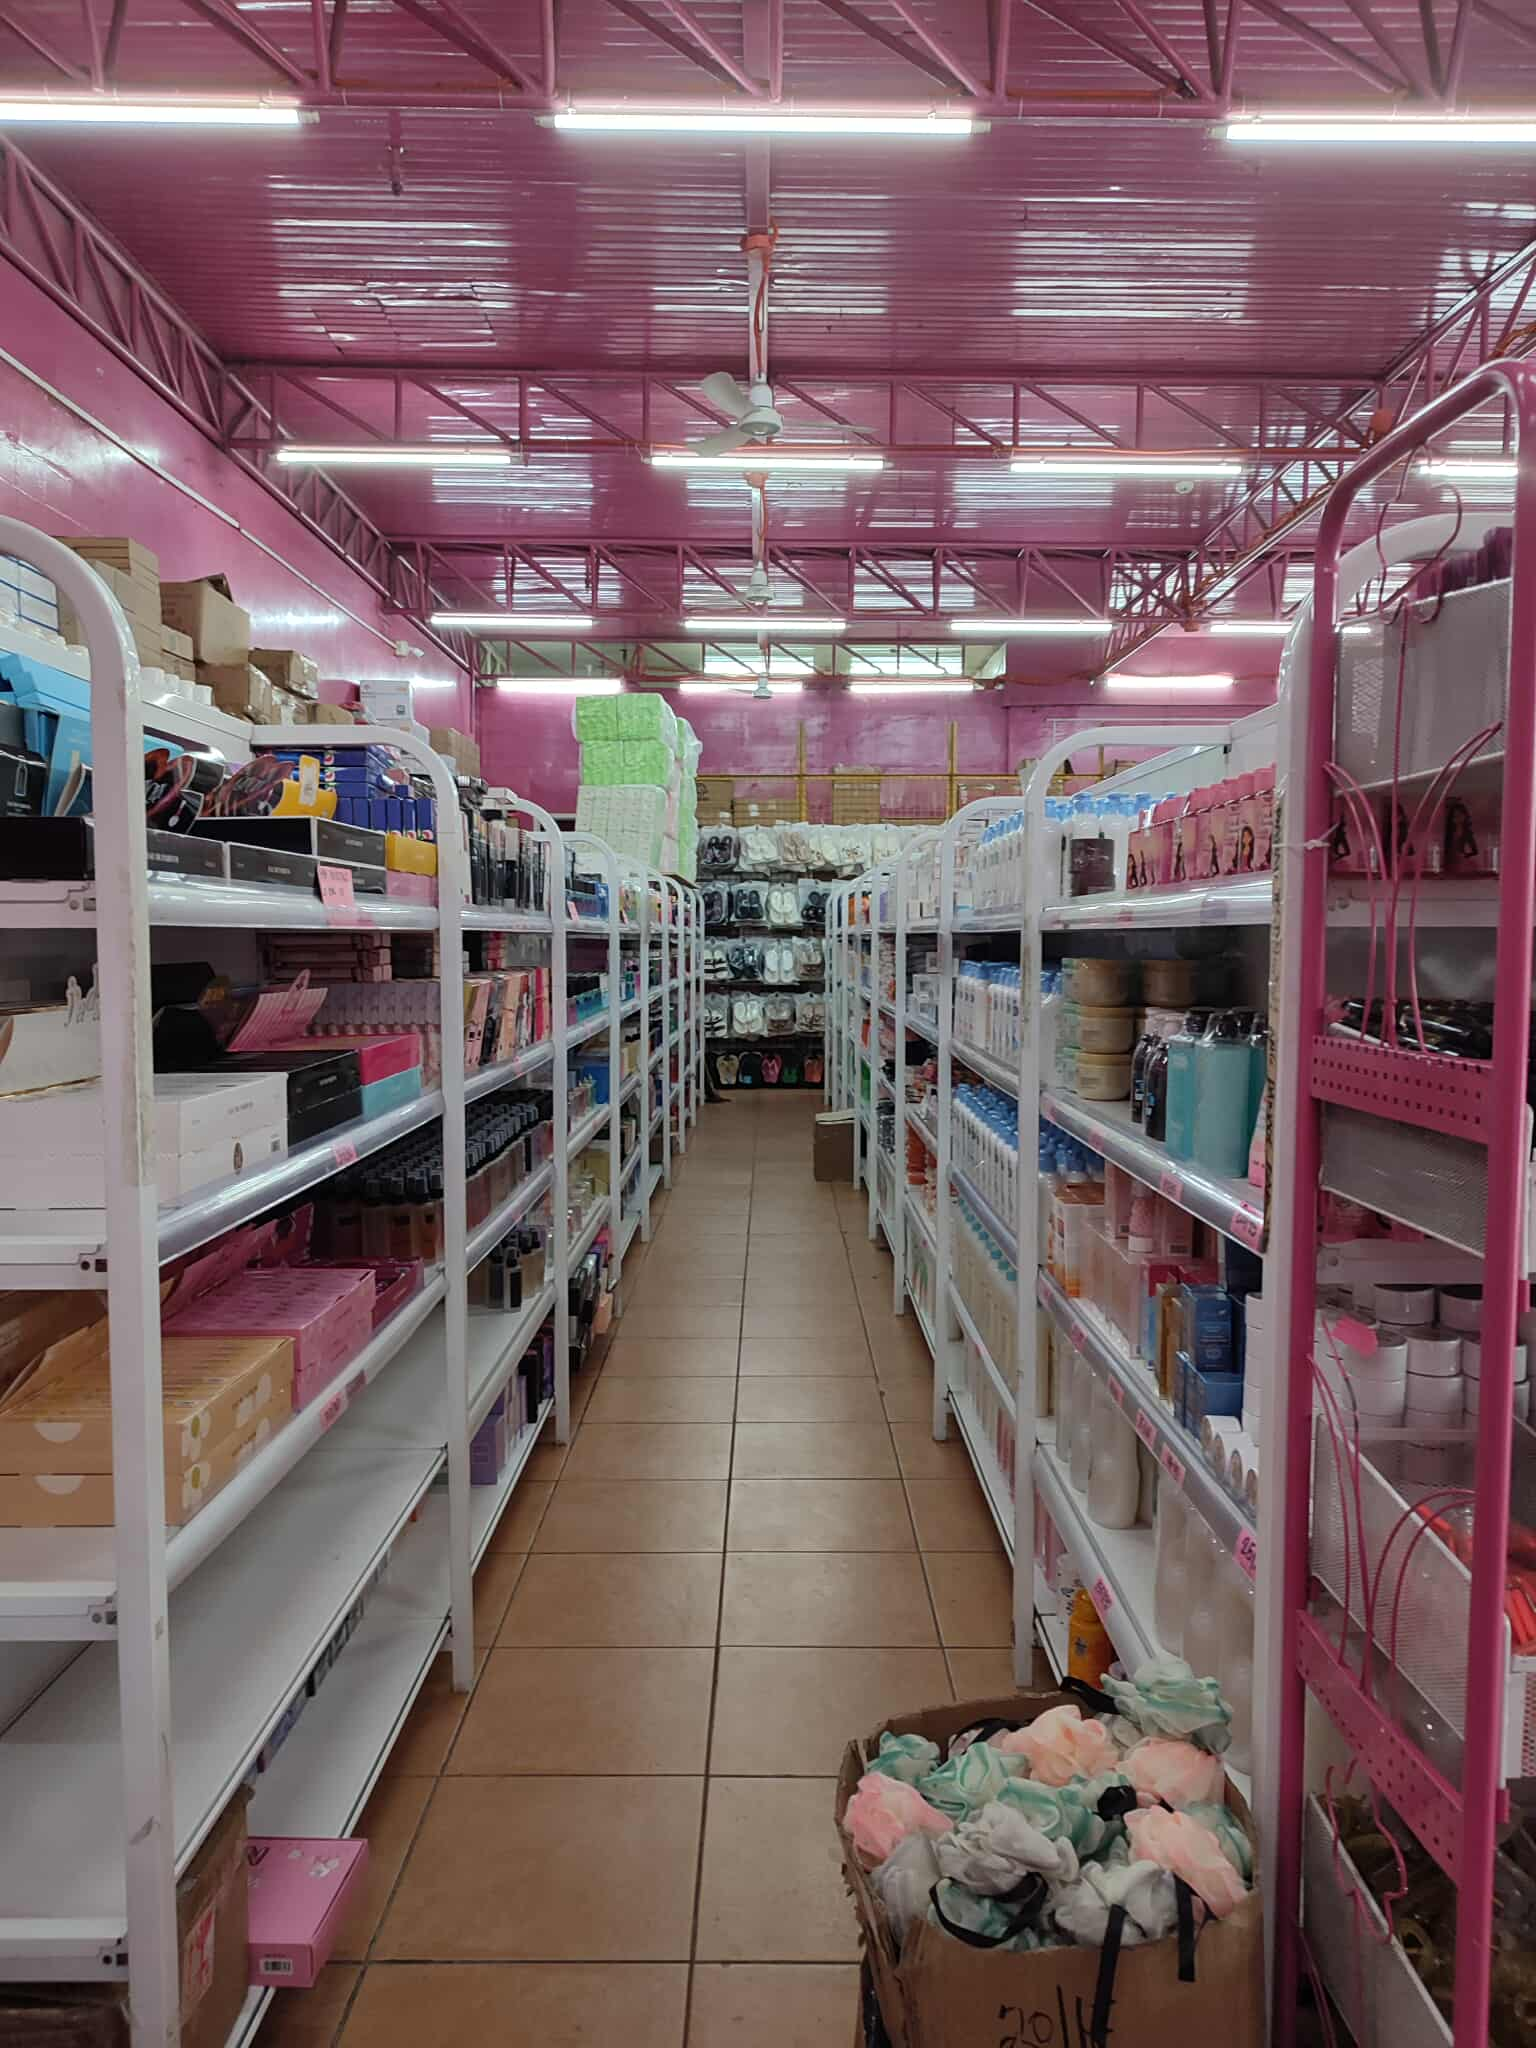
\includegraphics[width=0.30\textwidth]{appendices/zone2} \\
		\textbf{Beauty Zone: Body and Bath Products} & \textbf{Beauty Zone: Face and Hair Care Products} \\
		\textit{(Soap, Shampoo, Conditioner, etc.)} & \textit{(Perfumes, Hair Iron, Body Scrubs, etc.)} \\
		\hline
		\textbf{Zone C / Aisle 3} & \textbf{Zone D / Aisle 4} \\
		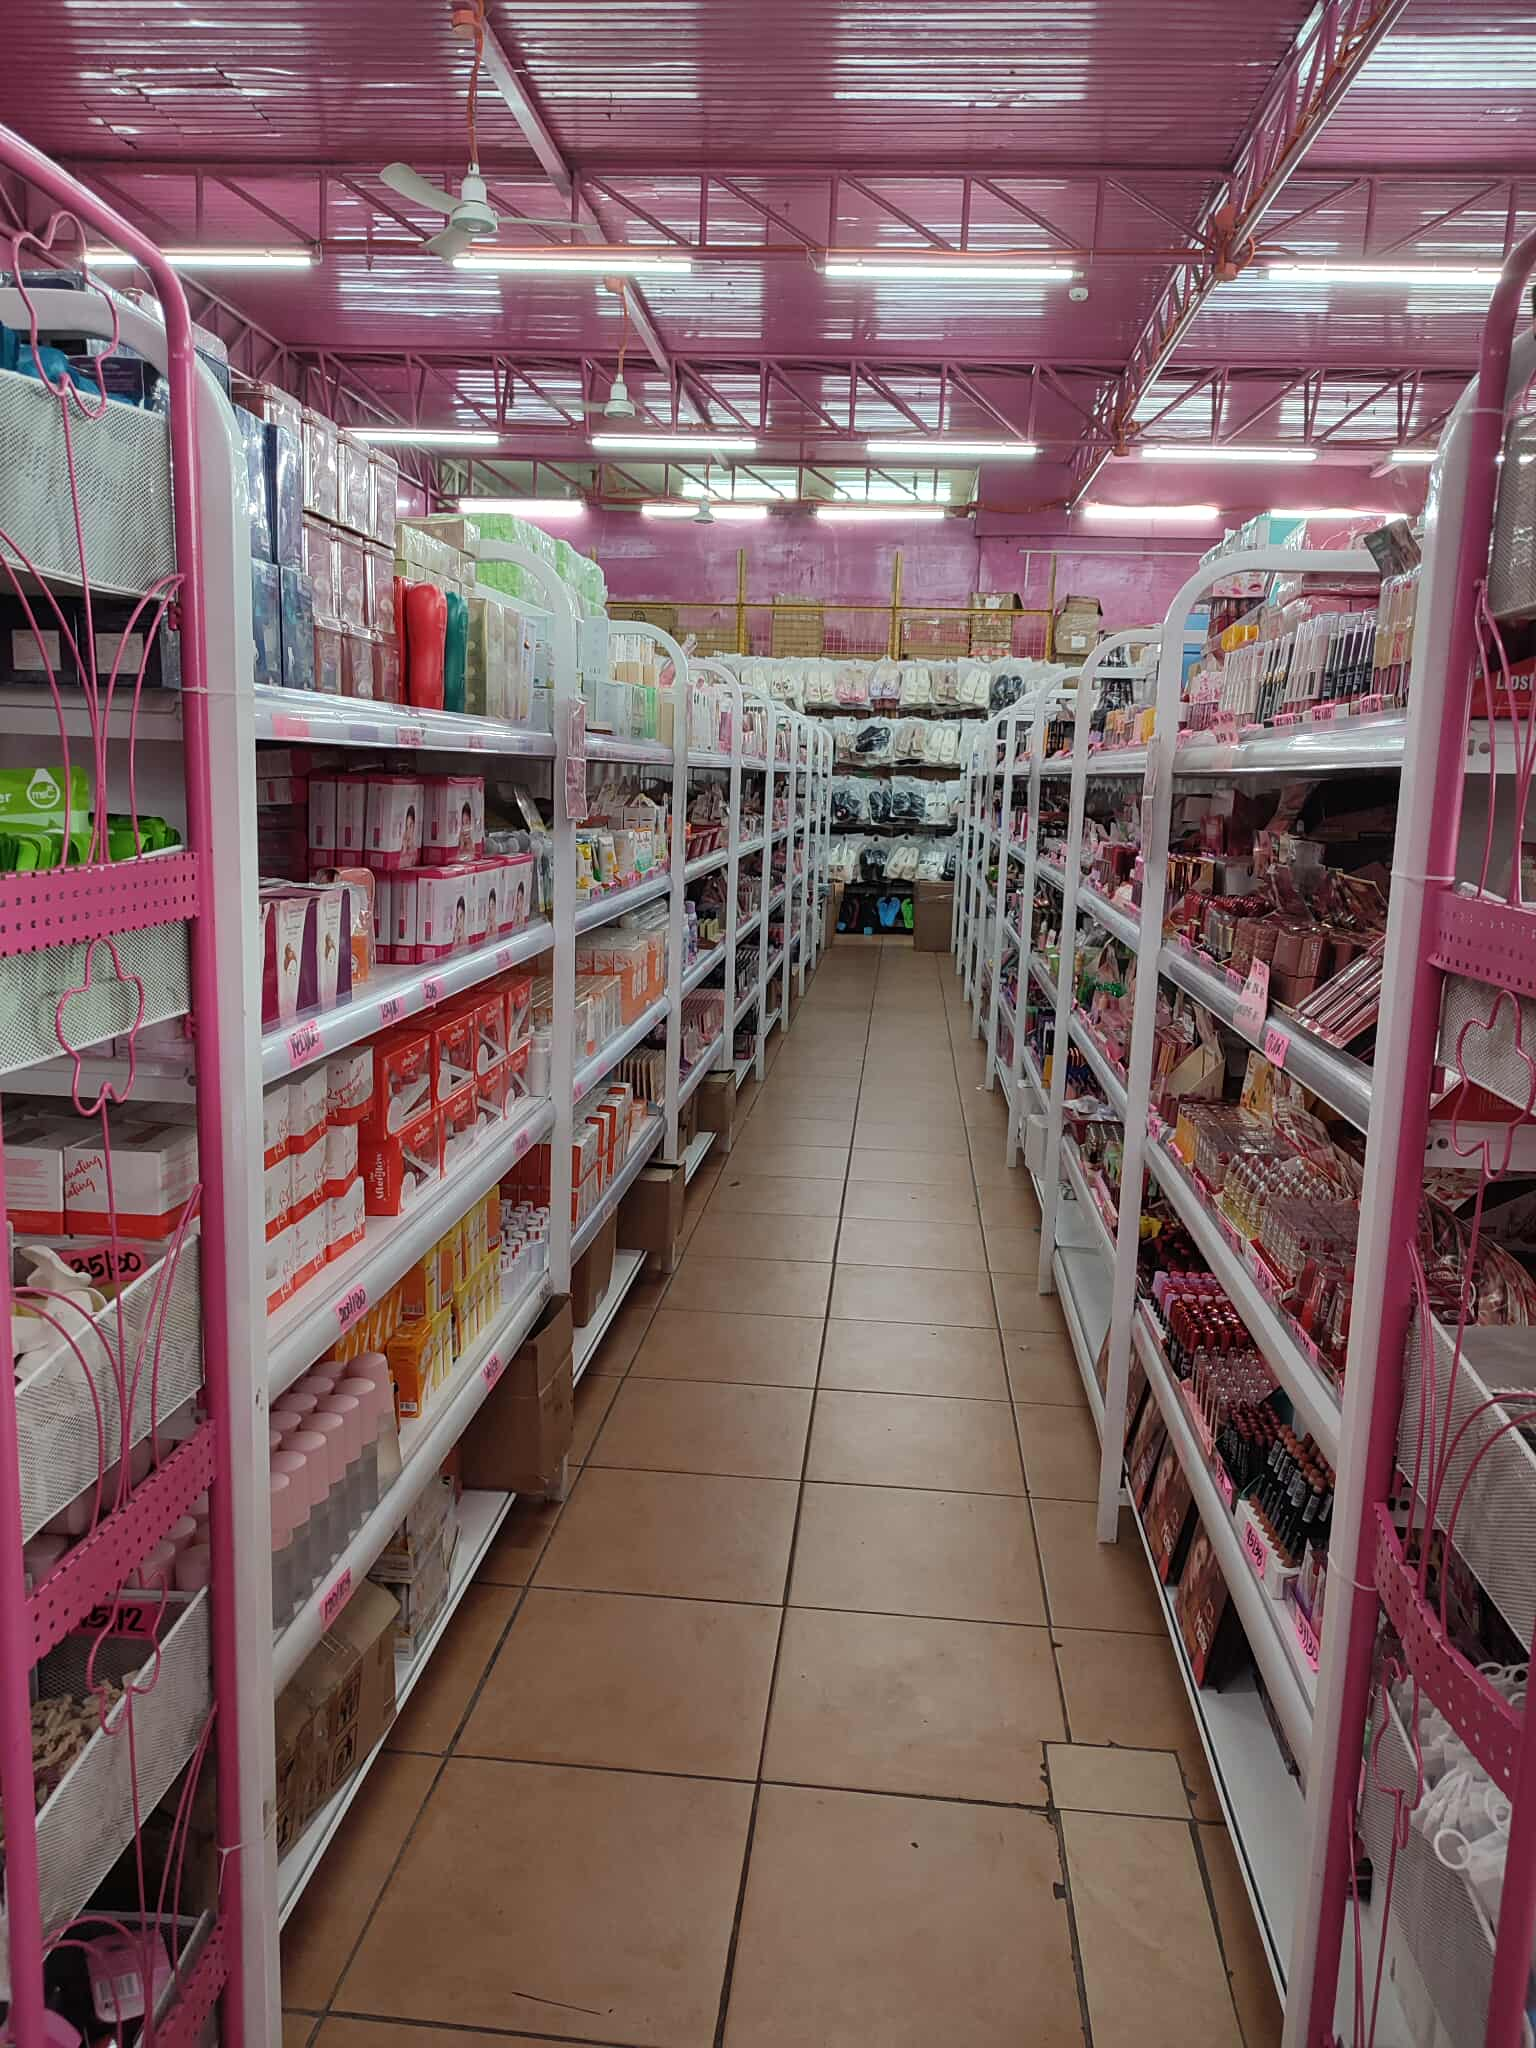
\includegraphics[width=0.30\textwidth]{appendices/zone3} & 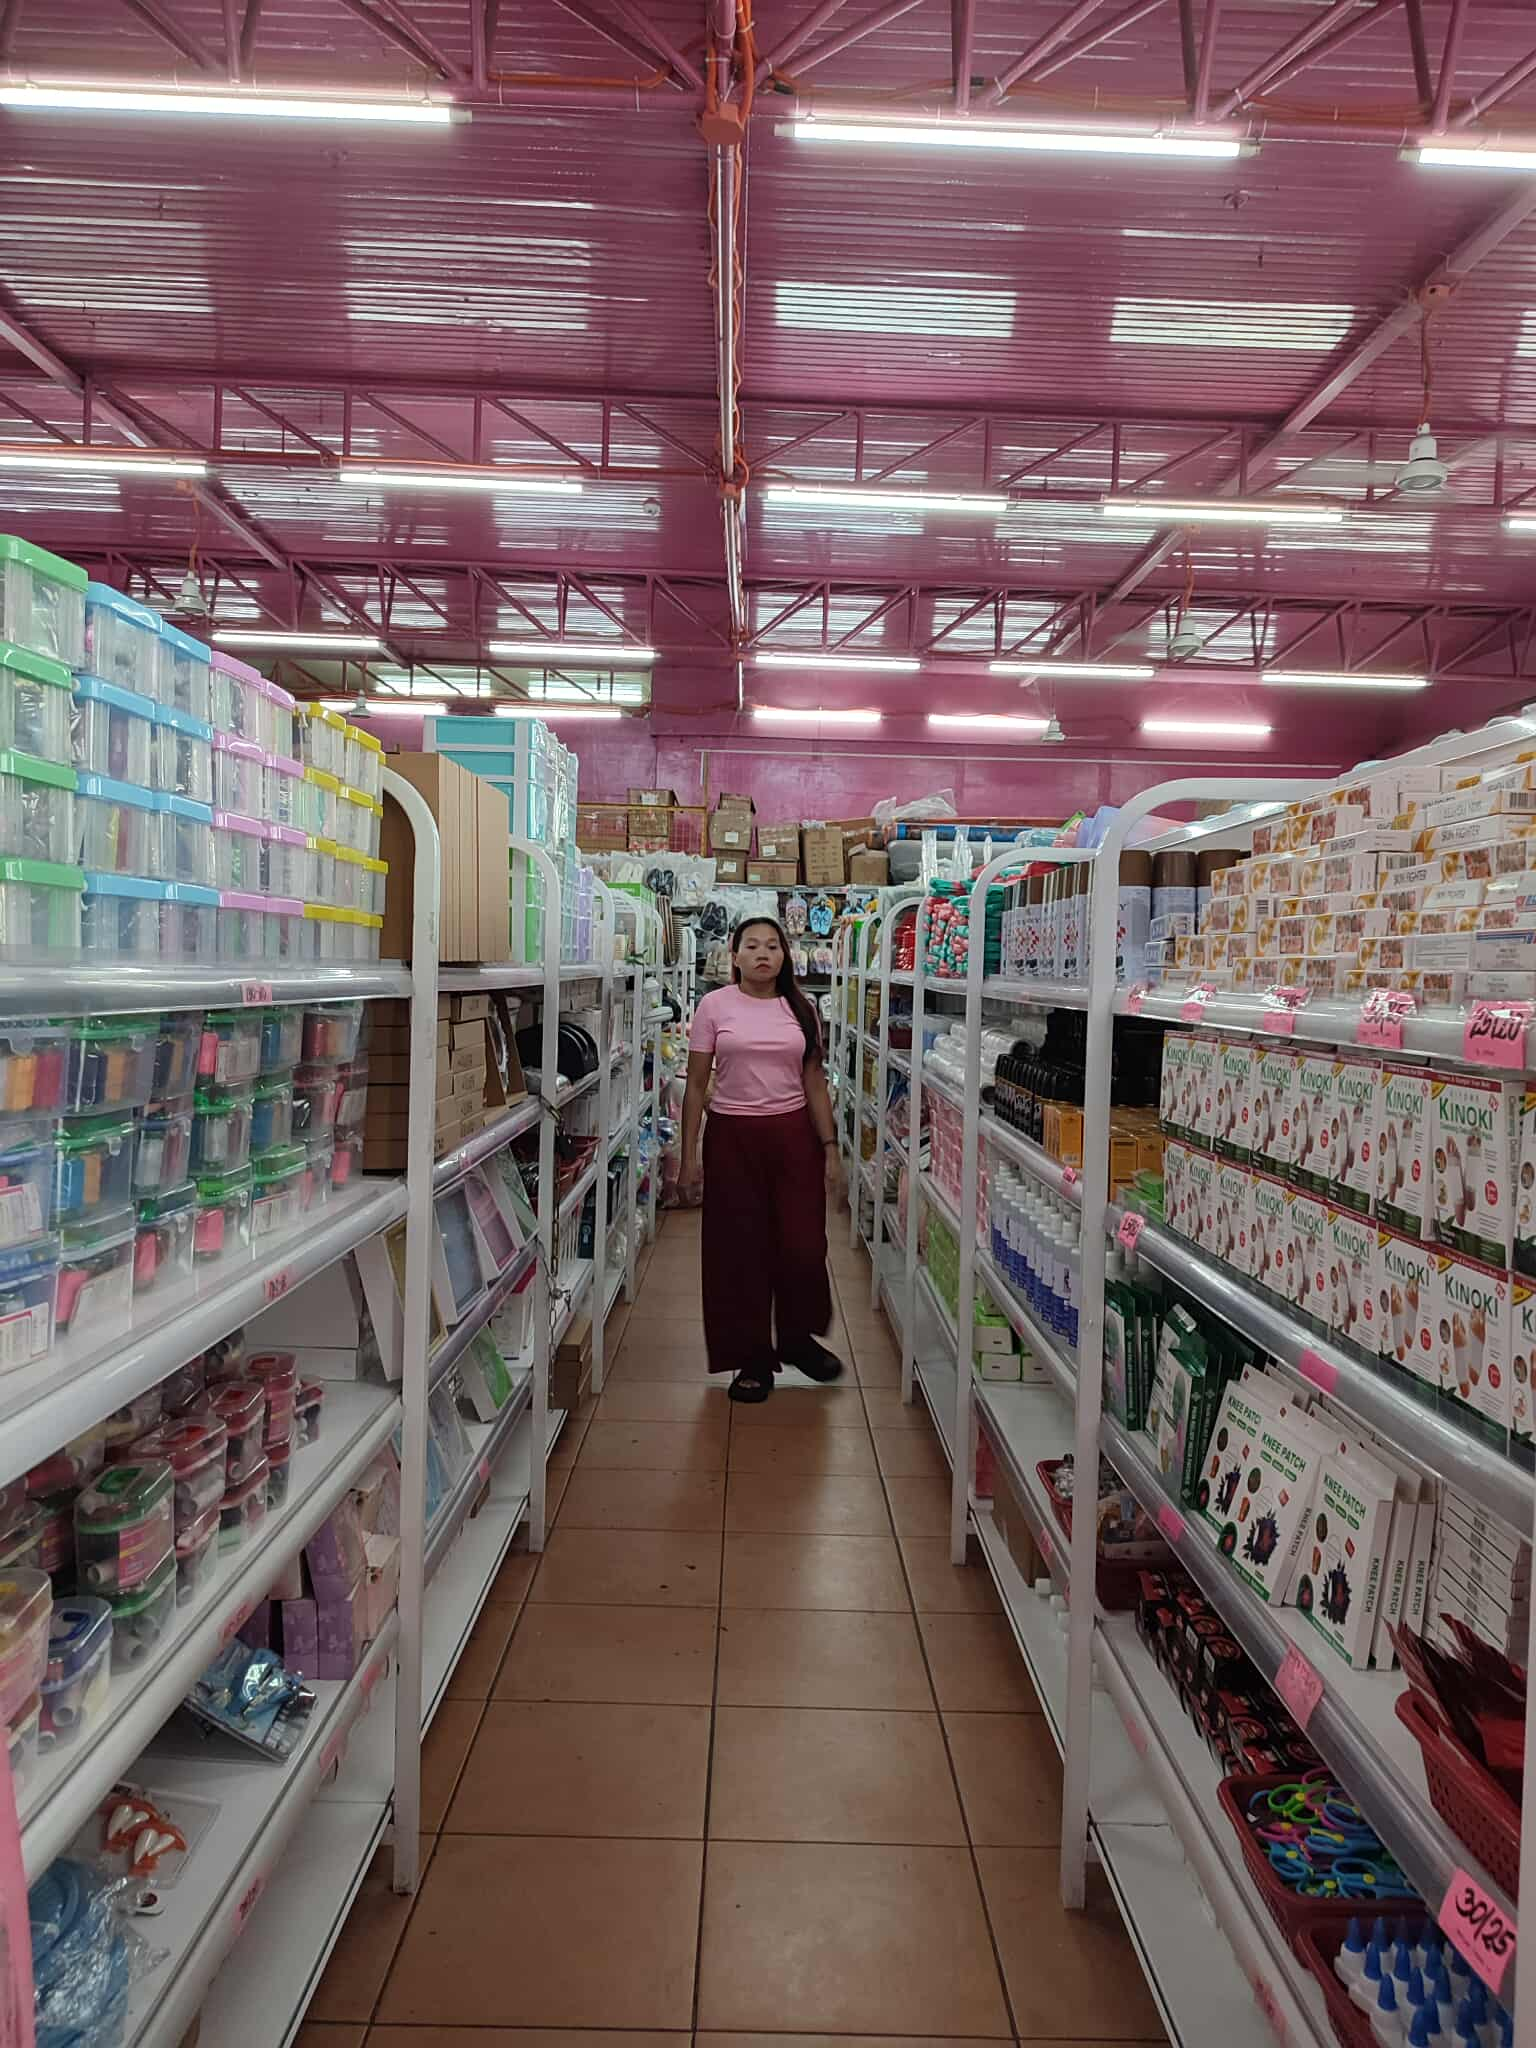
\includegraphics[width=0.30\textwidth]{appendices/zone4} \\
		\textbf{Beauty Zone: Cosmetics} & \textbf{Assorted Home Essentials} \\
		\textit{(Face Cleanser, Beauty Soap, Eye Makeup, etc.)} & \textit{(School Supplies, Sewing Kit, etc.)} \\
		\hline
		\textbf{Zone E / Aisle 5} & \textbf{Zone F / Aisle 6} \\
		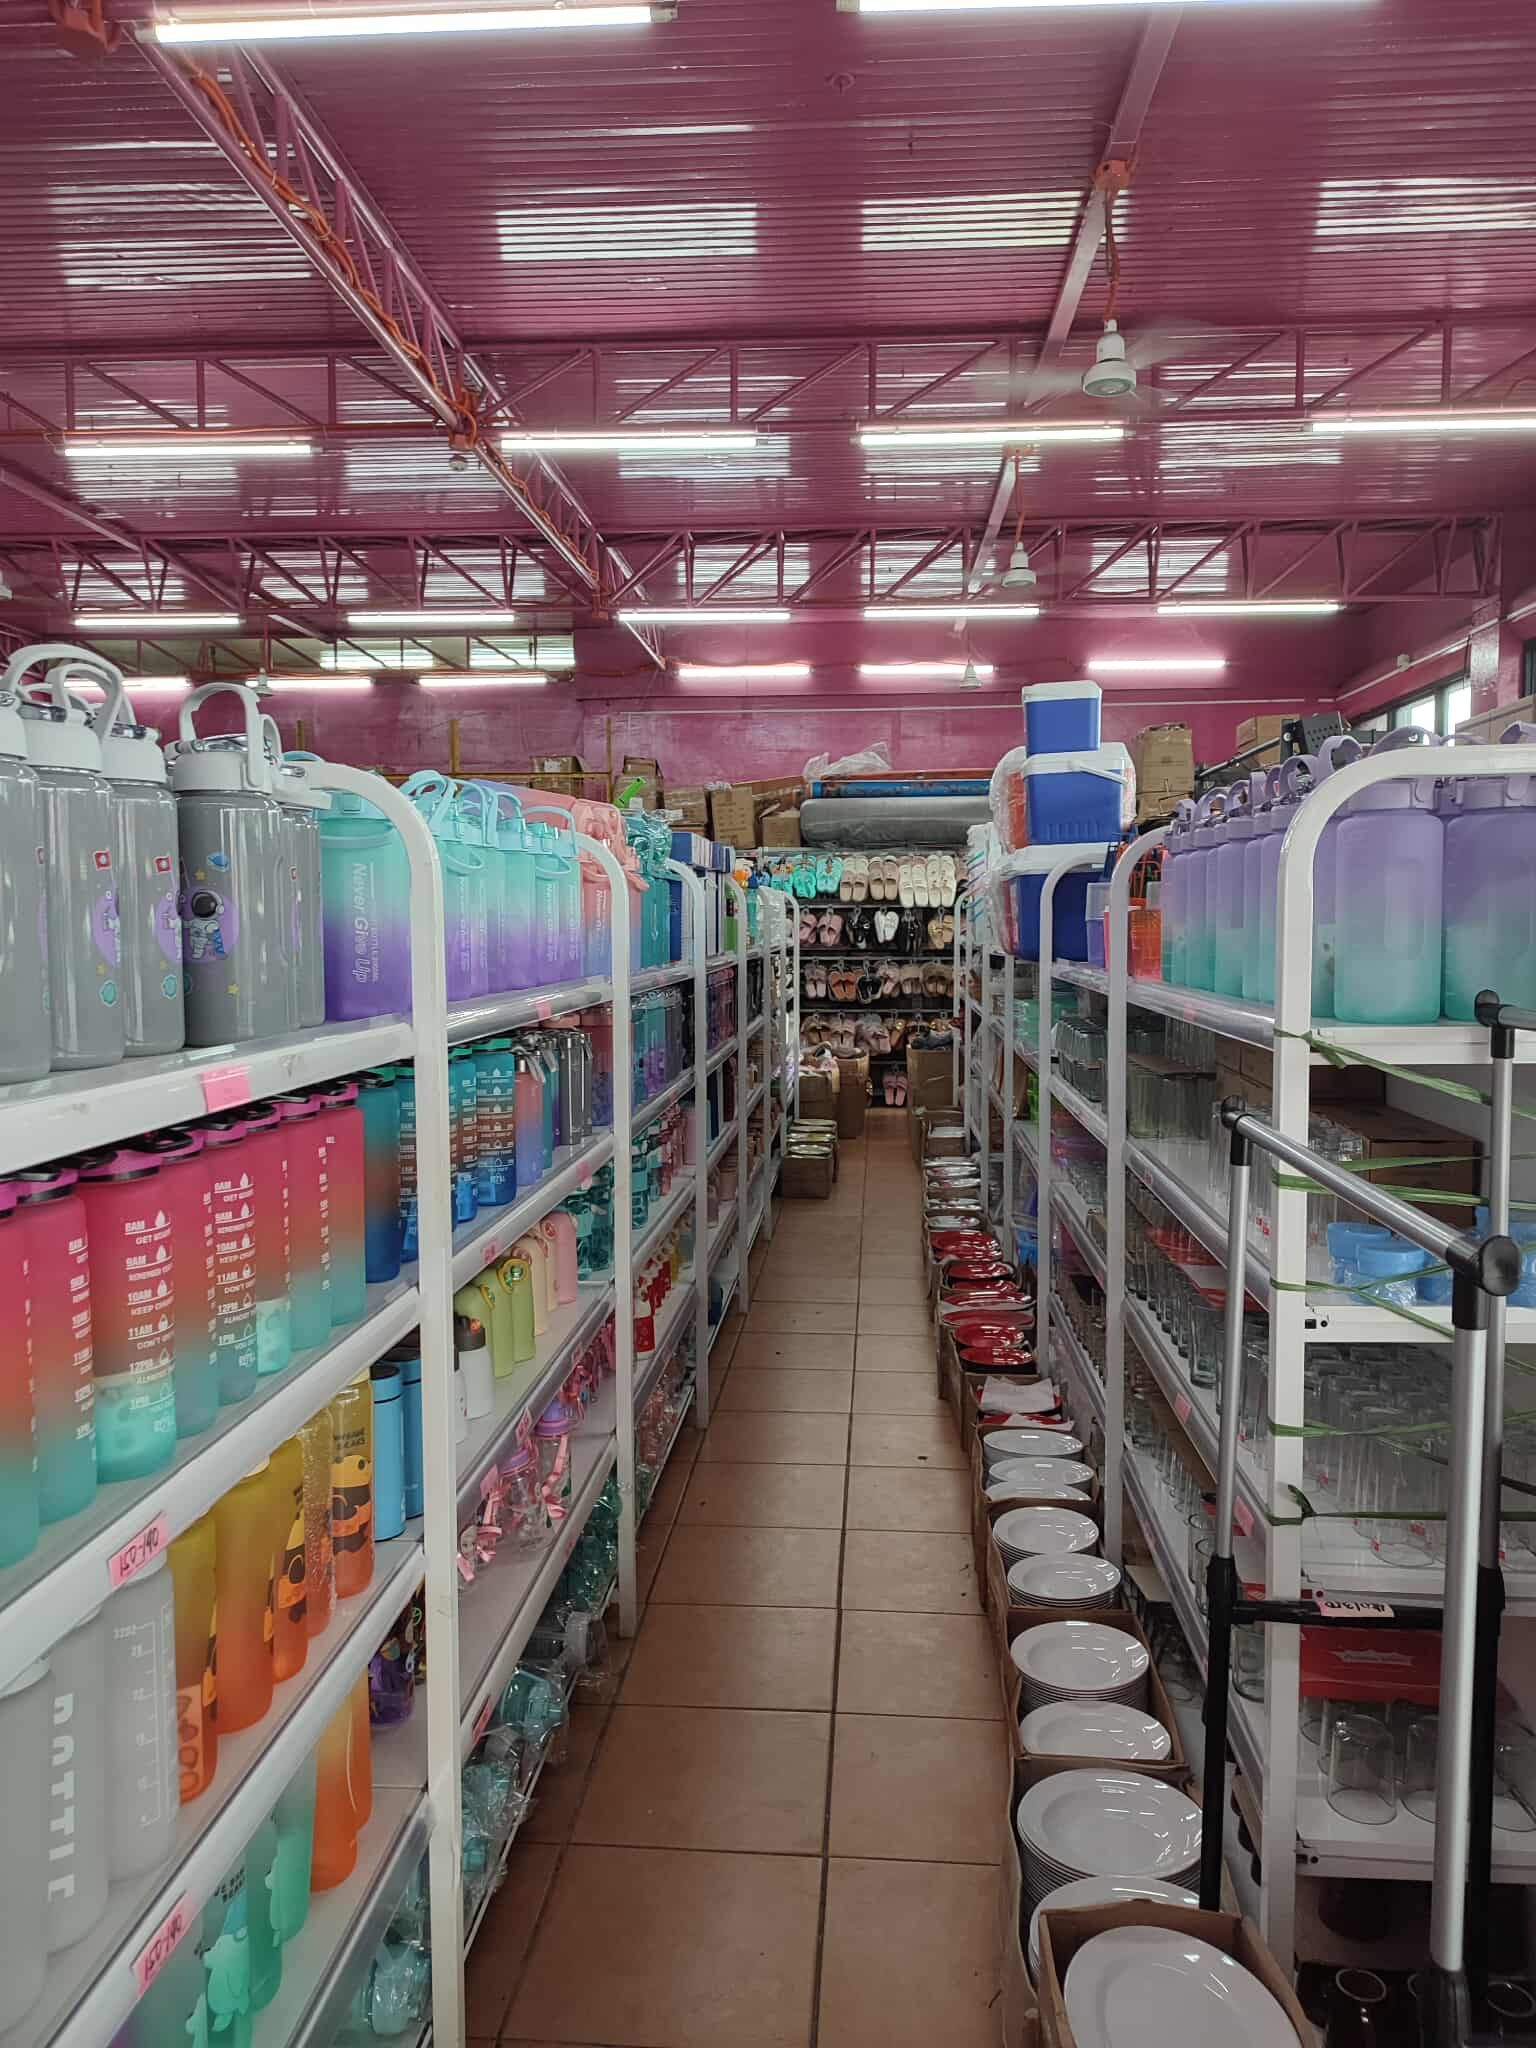
\includegraphics[width=0.30\textwidth]{appendices/zone5} & 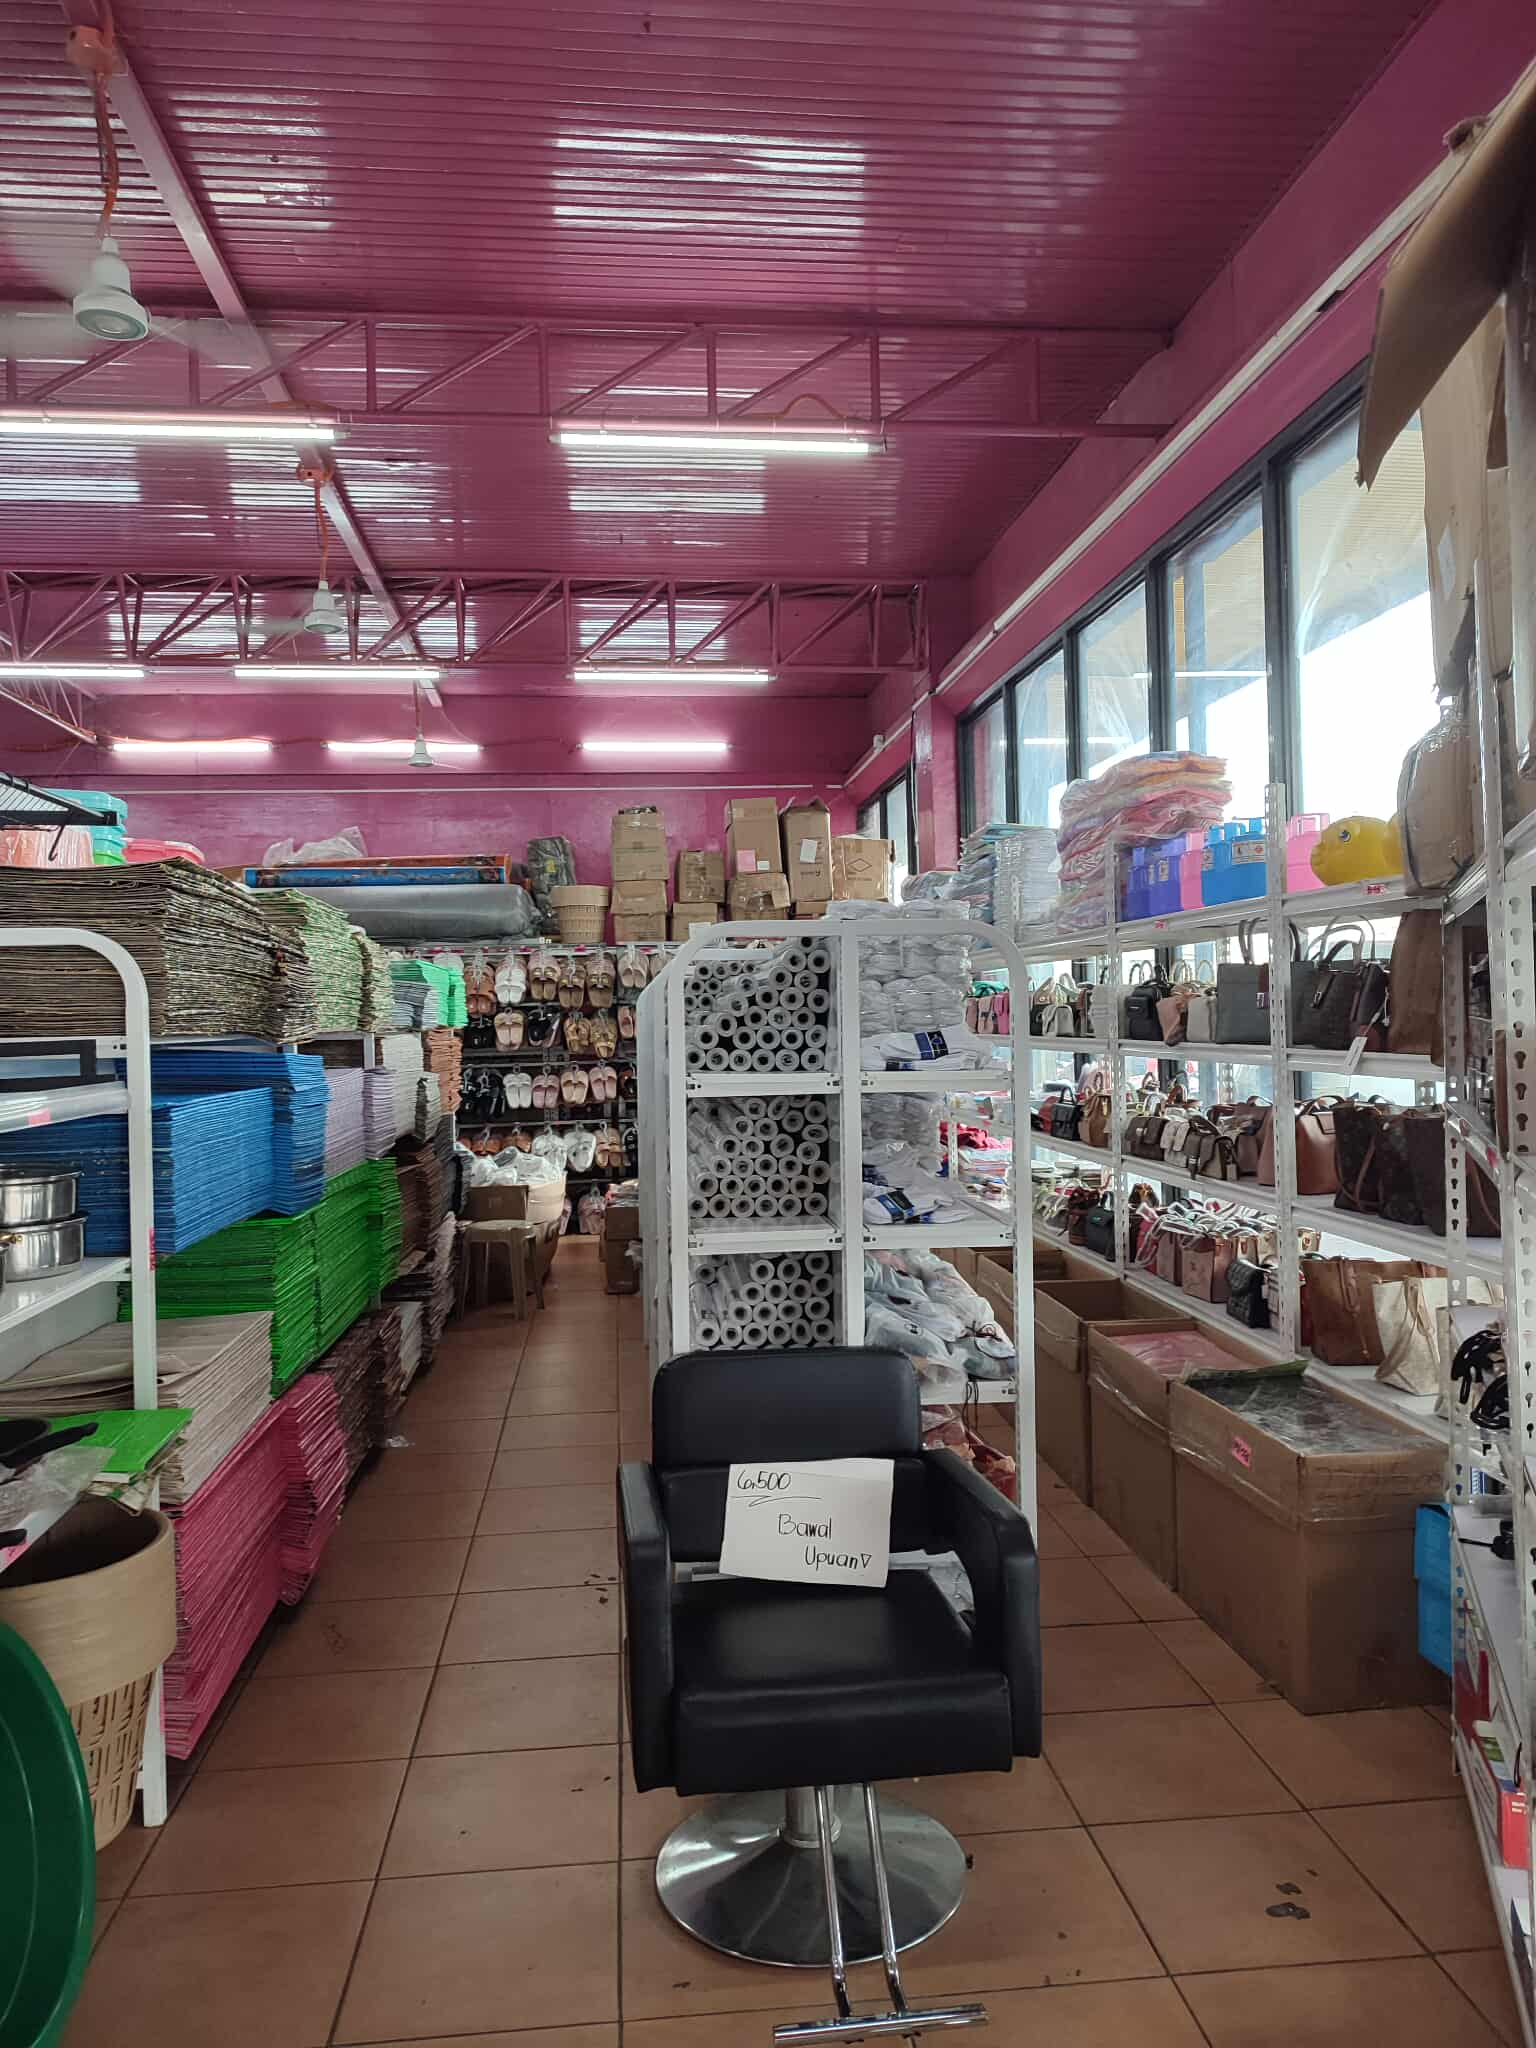
\includegraphics[width=0.30\textwidth]{appendices/zone6} \\
		\textbf{Kitchenwares} & \textbf{Home Products} \\
		\textit{(Tumbler, Containers, Plates, etc.)} & \textit{(Handbags, Floormat, Stickers, etc.)} \\
		\hline
	\end{longtable}
\end{center}

\clearpage

\begin{center}
	% Remove \thispagestyle{plain} to maintain consistent page numbering
	{\bf APPENDIX D}\\[24pt]
\end{center}
\addcontentsline{toc}{section}{APPENDIX D}

\begin{center}
	INTERVIEW CONDUCTED ON FASHIONLANE GIFT SHOP
\end{center}

\begin{center}
	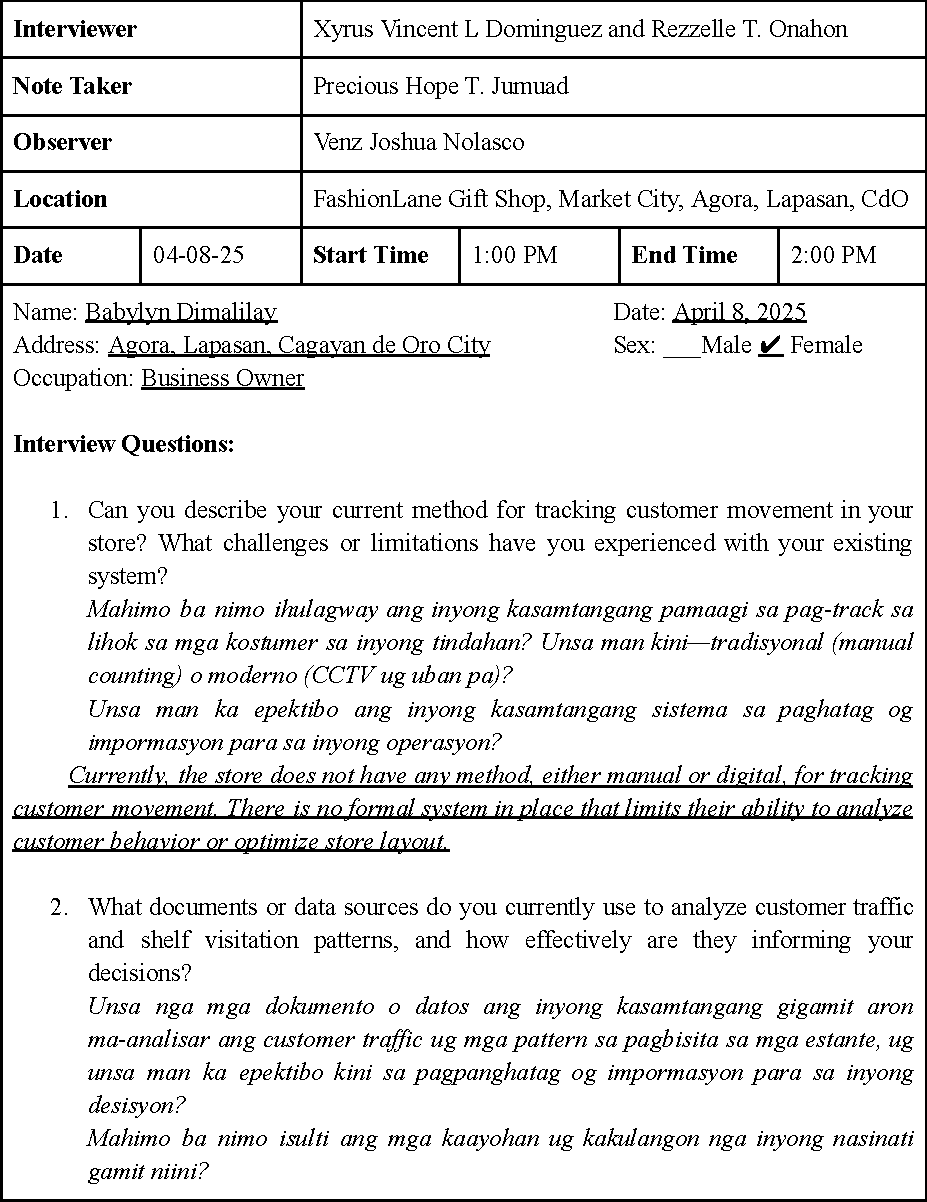
\includegraphics[width=0.95\textwidth]{app/D1.pdf}
	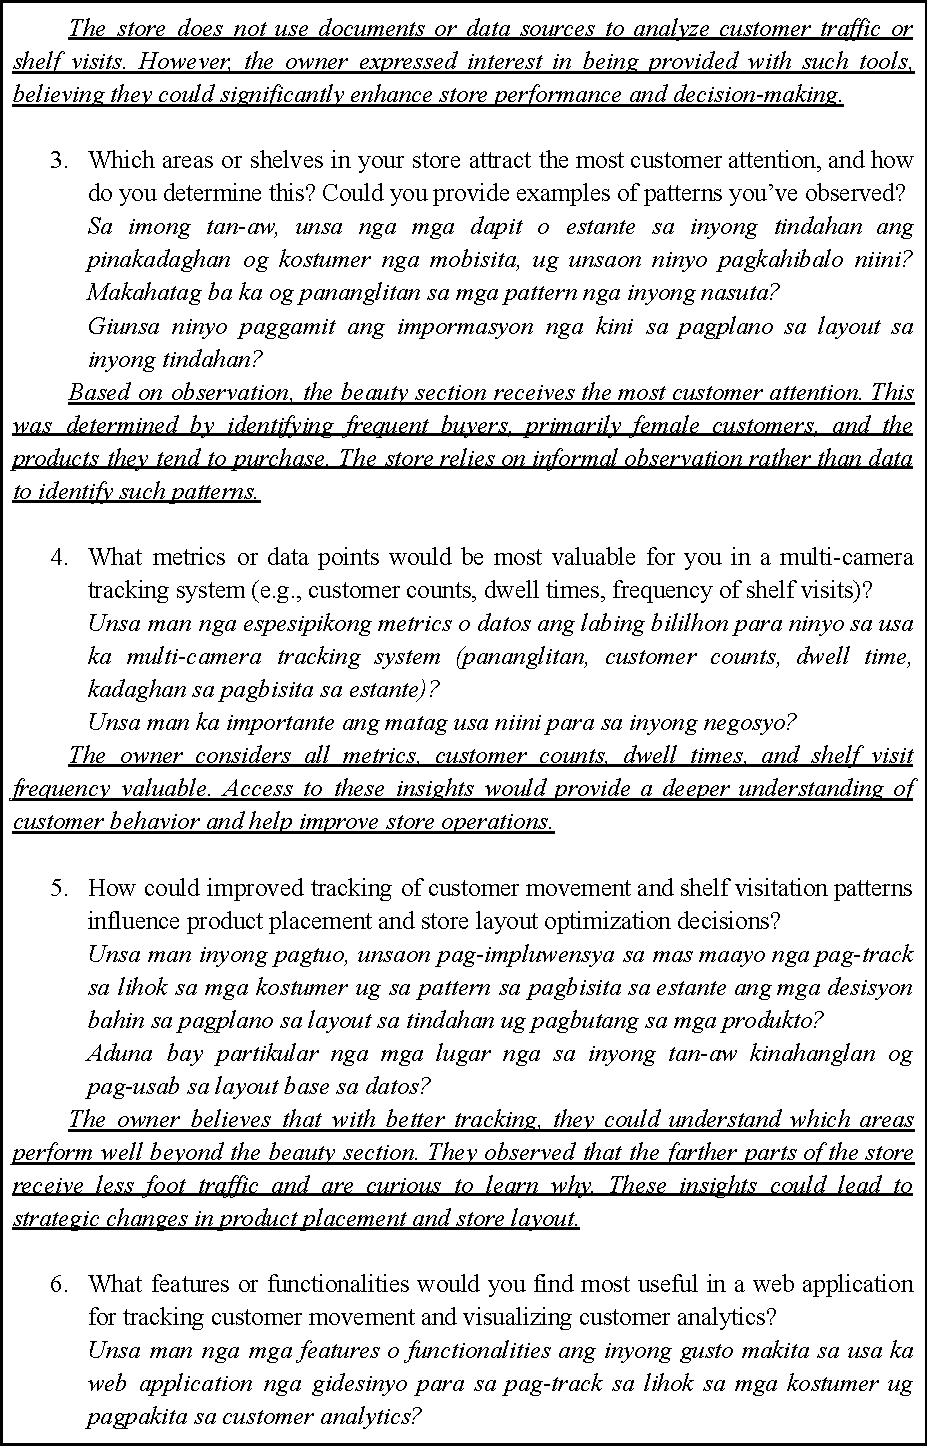
\includegraphics[width=0.92\textwidth]{app/D2.pdf}
	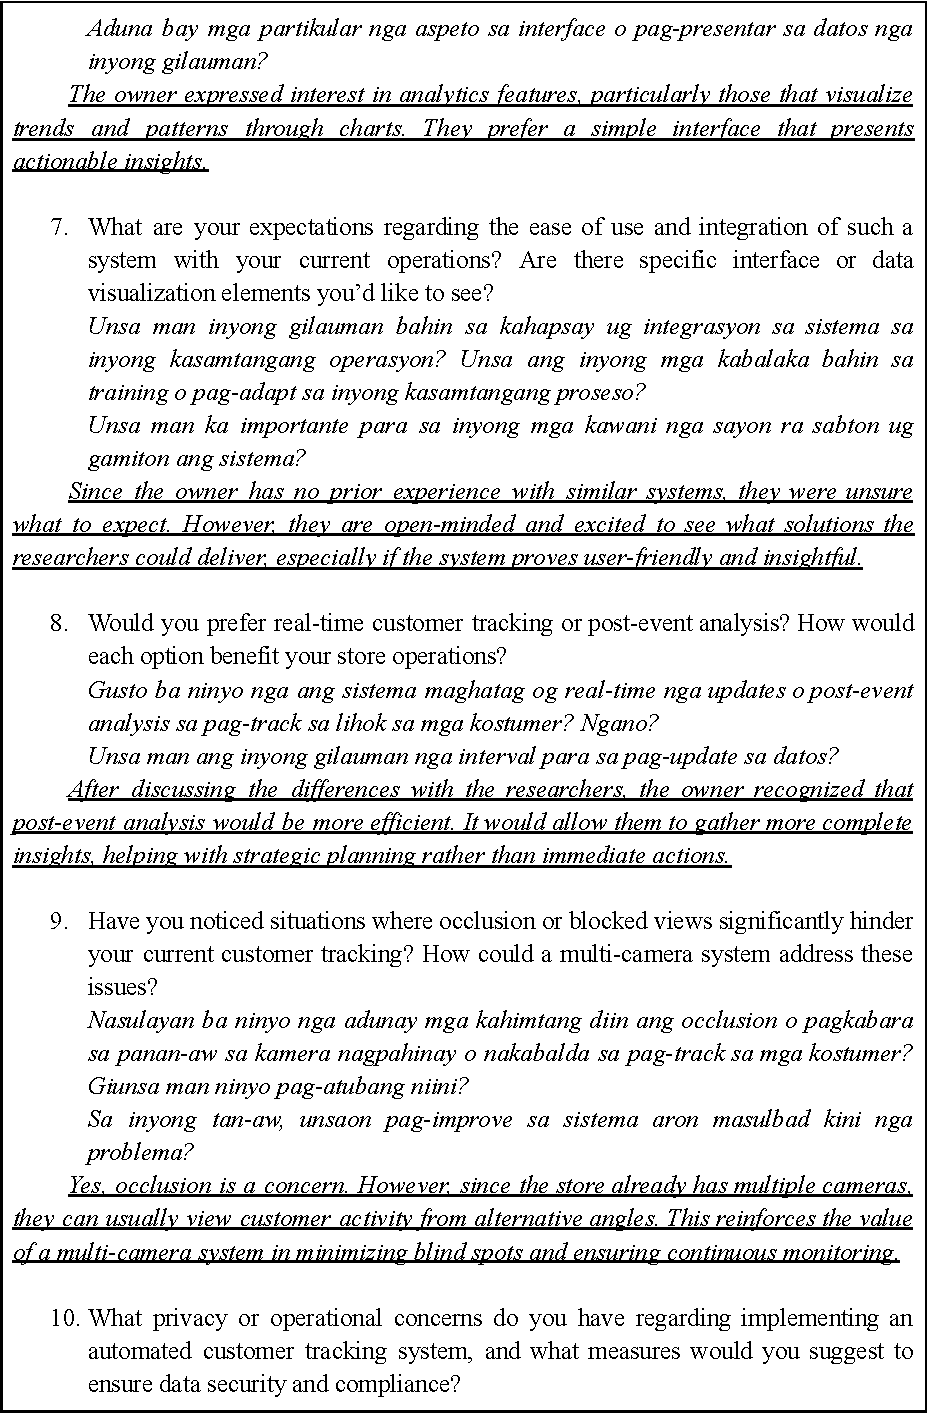
\includegraphics[width=0.92\textwidth]{app/D3.pdf}
	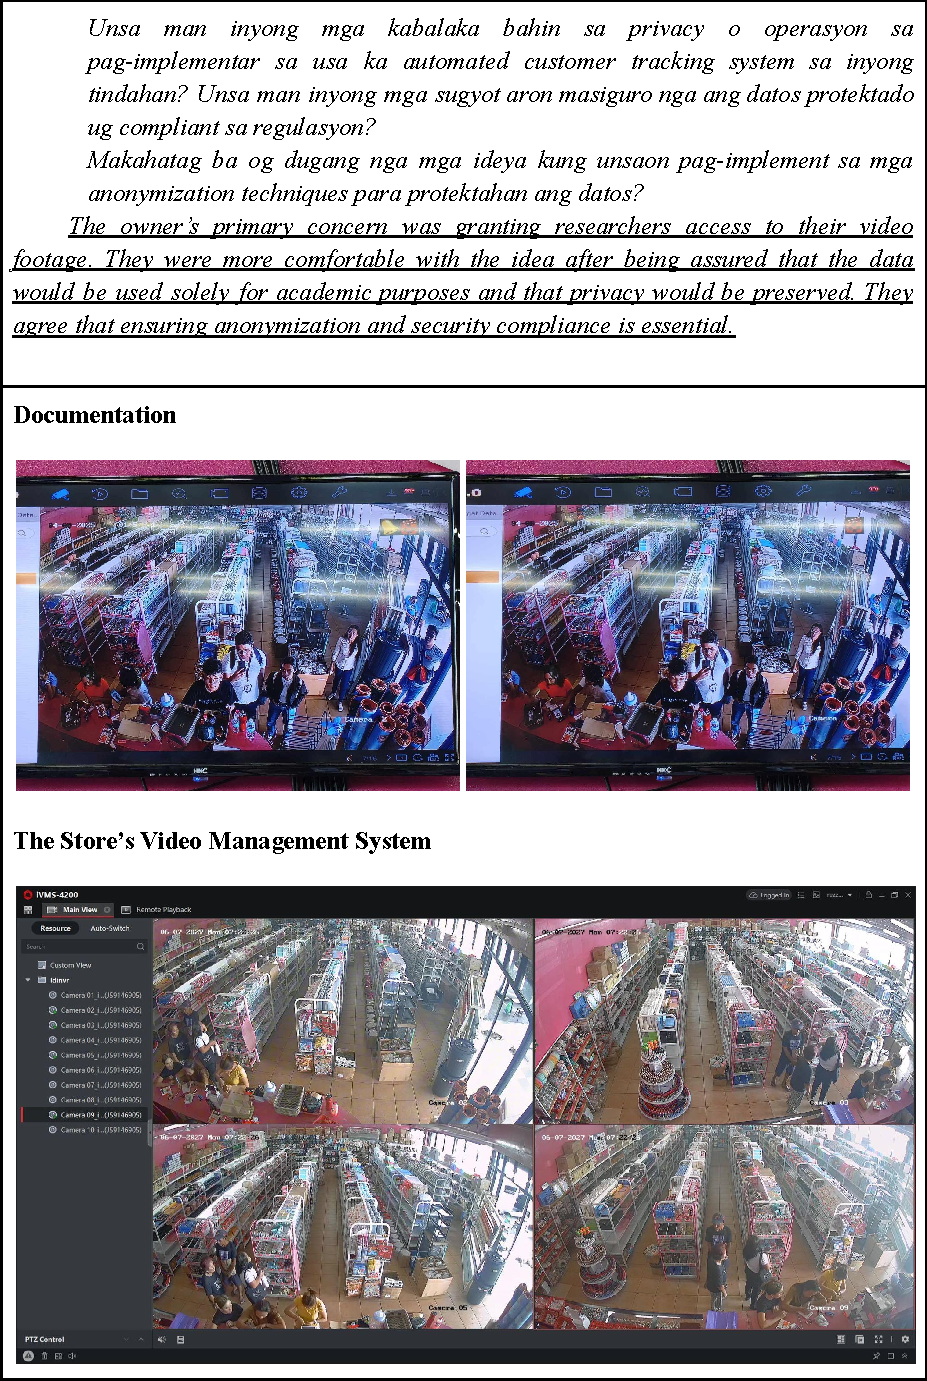
\includegraphics[width=0.92\textwidth]{app/D4.pdf}
\end{center}

\clearpage

\begin{center}
	% Remove \thispagestyle{plain} to maintain consistent page numbering
	{\bf APPENDIX E}\\[24pt]
\end{center}
\addcontentsline{toc}{section}{APPENDIX E}

\begin{center}
	RE-IDENTIFICATION AND HEAT MAPPING RUNS ACROSS ALL ZONES IN ALL FOUR CAMERAS
\end{center}

\begin{center}
	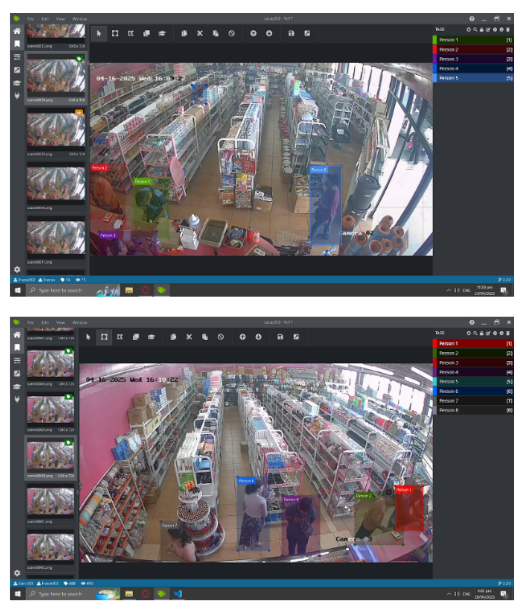
\includegraphics[width=0.90\textwidth]{app/E.pdf}
\end{center}

\clearpage

\begin{center}
	% Remove \thispagestyle{plain} to maintain consistent page numbering
	{\bf APPENDIX F}\\[24pt]
\end{center}
\addcontentsline{toc}{section}{APPENDIX F}

\begin{center}
	FUNCTIONAL TEST RESULT OF STORE OWNER/MANAGER (n=1)
\end{center}

\begin{center}
	\noindent
	\resizebox{\textwidth}{!}{%
		\begin{tabular}{|c|p{10cm}|c|c|}
			\hline
			\textbf{No.} & \textbf{Description} & \textbf{Frequency} & \textbf{Percentage} \\
			\hline
			1 & Could the system accept and display video feeds from the existing CCTV infrastructure? & 1 & 100 \\
			\hline
			2 & Did the system detect and highlight customers entering the store on the feed? & 1 & 100 \\
			\hline
			3 & Did the system consistently track customer movement across different store zones? & 1 & 100 \\
			\hline
			4 & Was the system able to detect when customers interacted with shelves or display zones? & 1 & 100 \\
			\hline
			5 & Did the system automatically log customer entries, exits, and dwell times without manual intervention? & 1 & 100 \\
			\hline
			6 & Did the system assign and maintain unique tracking IDs to customers throughout their store journey? & 1 & 100 \\
			\hline
			7 & Was customer behavioral data (e.g., foot traffic, dwell time) displayed correctly and clearly on the dashboard? & 1 & 100 \\
			\hline
			8 & Could the user view foot traffic heat maps and generate behavioral trend charts from the collected data? & 1 & 100 \\
			\hline
			9 & Was access restricted through an admin login, and was no personally identifiable information (PII) collected or displayed? & 1 & 100 \\
			\hline
			10 & Did the system maintain responsive performance even when handling multiple video streams simultaneously? & 1 & 100 \\
			\hline
		\end{tabular}%
	}
	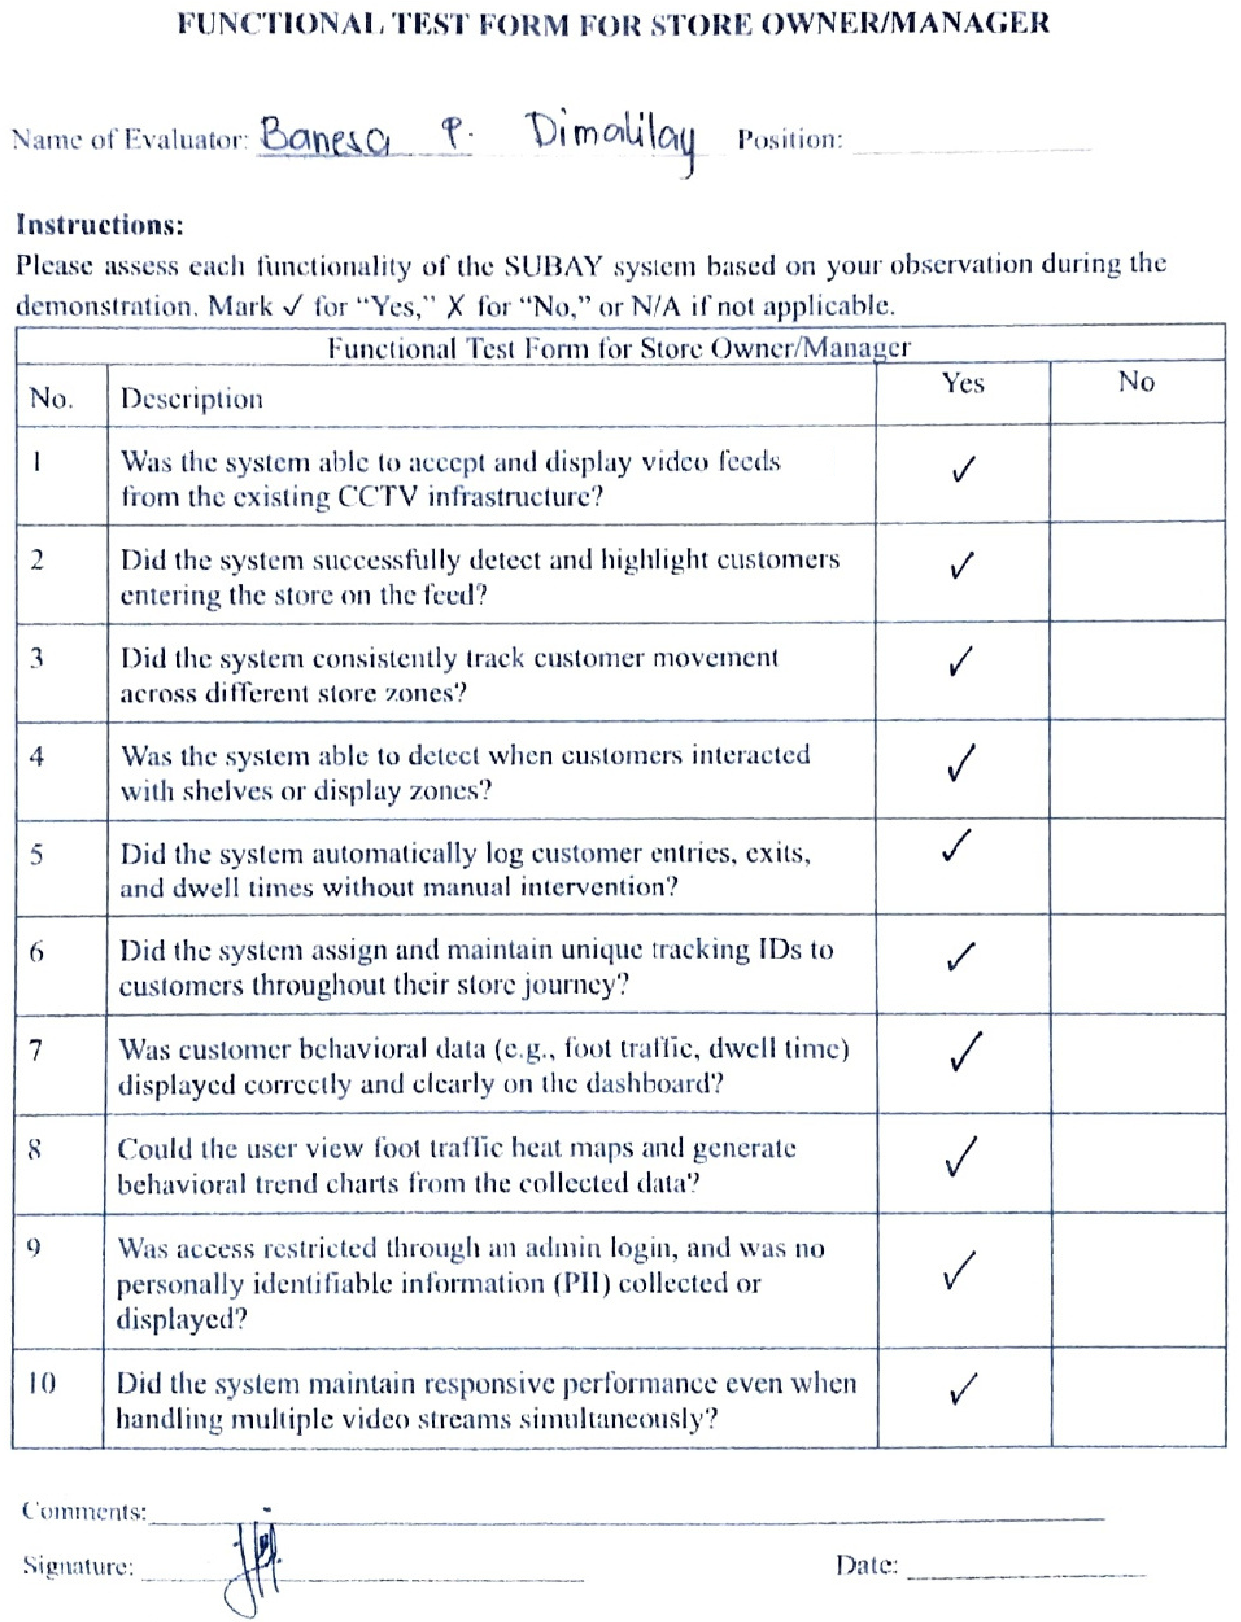
\includegraphics[width=1\textwidth]{app/F.pdf}
\end{center}

\clearpage

\begin{center}
	% Remove \thispagestyle{plain} to maintain consistent page numbering
	{\bf APPENDIX G}\\[24pt]
\end{center}
\addcontentsline{toc}{section}{APPENDIX G}

\begin{center}
	SYSTEM USABILITY SCALE RESULT OF RETAIL OWNER/MANAGER (n=1)
\end{center}

\begin{center}
	\begin{tabular}{|c|p{8cm}|c|c|c|c|c|}
		\hline
		\multicolumn{7}{|c|}{\textbf{System Usability Scale}} \\
		\hline
		\multirow{2}{*}{No.} & \multirow{2}{*}{Item} & \multicolumn{5}{c|}{Frequency} \\
		\cline{3-7}
		& & SD & D & N & A & SA \\
		\hline
		1 & I think that I would like to use this system frequently & 0 & 0 & 0 & 1 & 0 \\
		\hline
		2 & I found the system unnecessarily complex & 0 & 1 & 0 & 0 & 0 \\
		\hline
		3 & I thought the system was easy to use & 0 & 0 & 0 & 0 & 1 \\
		\hline
		4 & I think that I would need the support of a technical person to be able to use this system & 1 & 0 & 0 & 0 & 0 \\
		\hline
		5 & I found that the various functions in this system were well integrated & 0 & 0 & 0 & 0 & 1 \\
		\hline
		6 & I thought there was too much inconsistency in this system & 1 & 0 & 0 & 0 & 0 \\
		\hline
		7 & I would imagine that most people would learn to use this system very quickly & 0 & 0 & 0 & 1 & 0 \\
		\hline
		8 & I found the system very cumbersome to use & 0 & 0 & 0 & 0 & 0 \\
		\hline
		9 & I felt very confident using the system & 0 & 0 & 0 & 1 & 0 \\
		\hline
		10 & I needed to learn a lot of things before I could get going with this system & 1 & 0 & 0 & 0 & 0 \\
		\hline
	\end{tabular}
	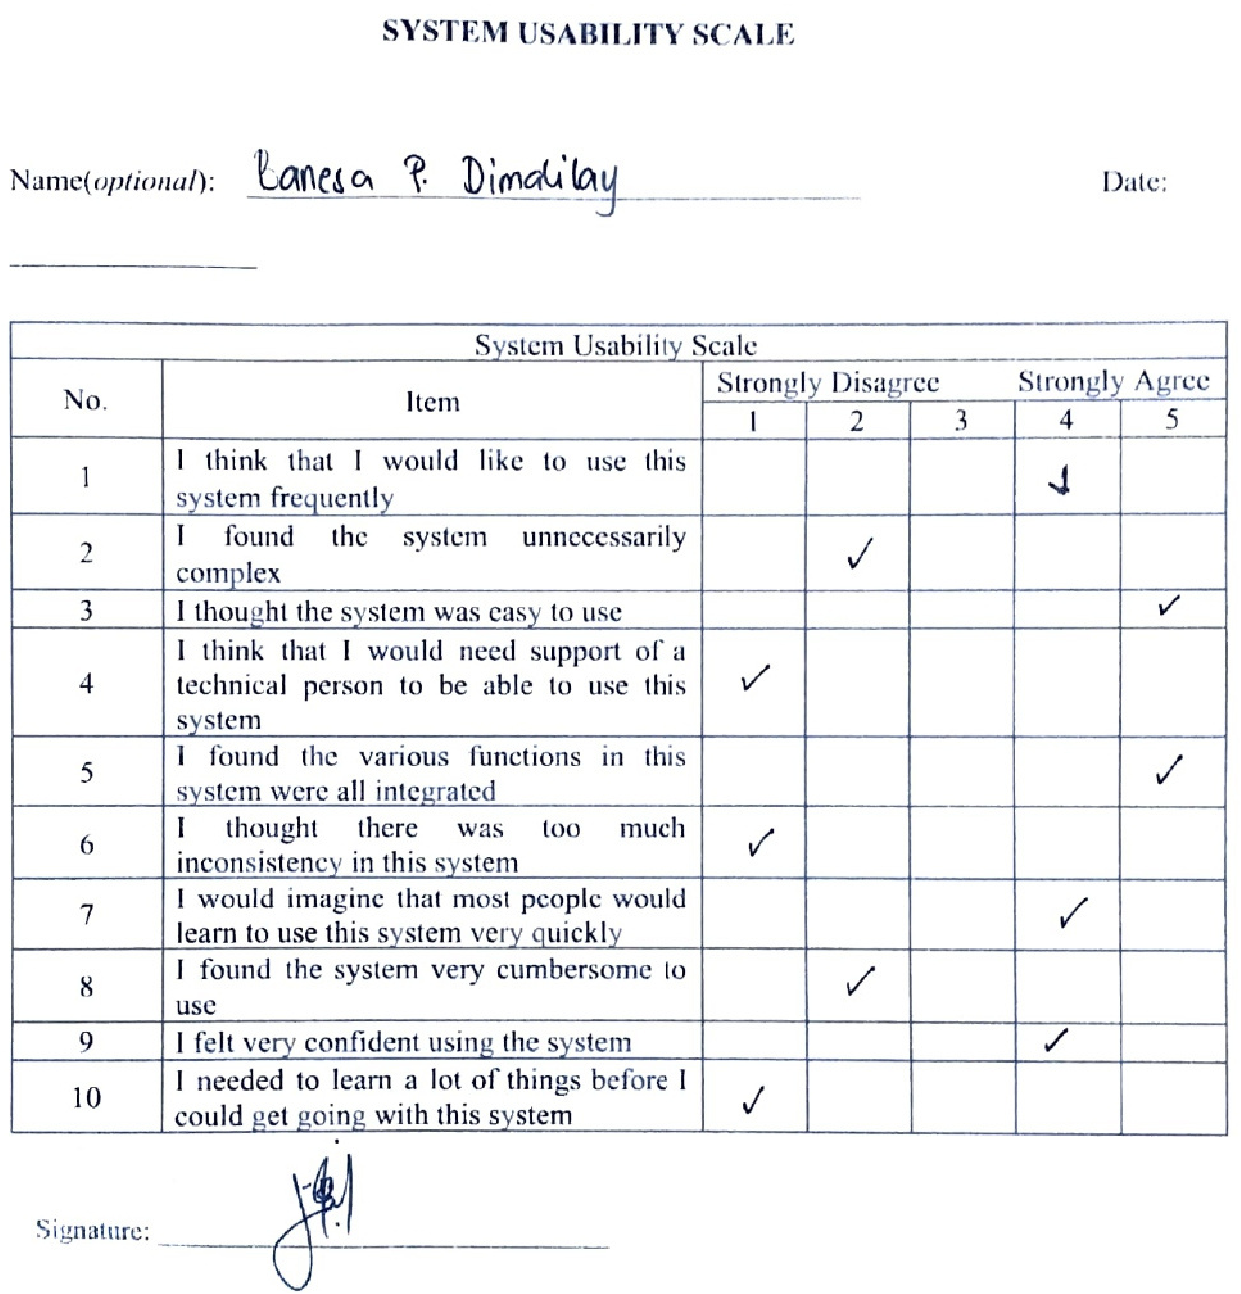
\includegraphics[width=1\textwidth]{app/G.pdf}
\end{center}

\clearpage

\begin{center}
	% Remove \thispagestyle{plain} to maintain consistent page numbering
	{\bf APPENDIX H}\\[24pt]
\end{center}
\addcontentsline{toc}{section}{APPENDIX H}

\begin{center}
	TRAINING CONDUCTED
\end{center}

\begin{center}
	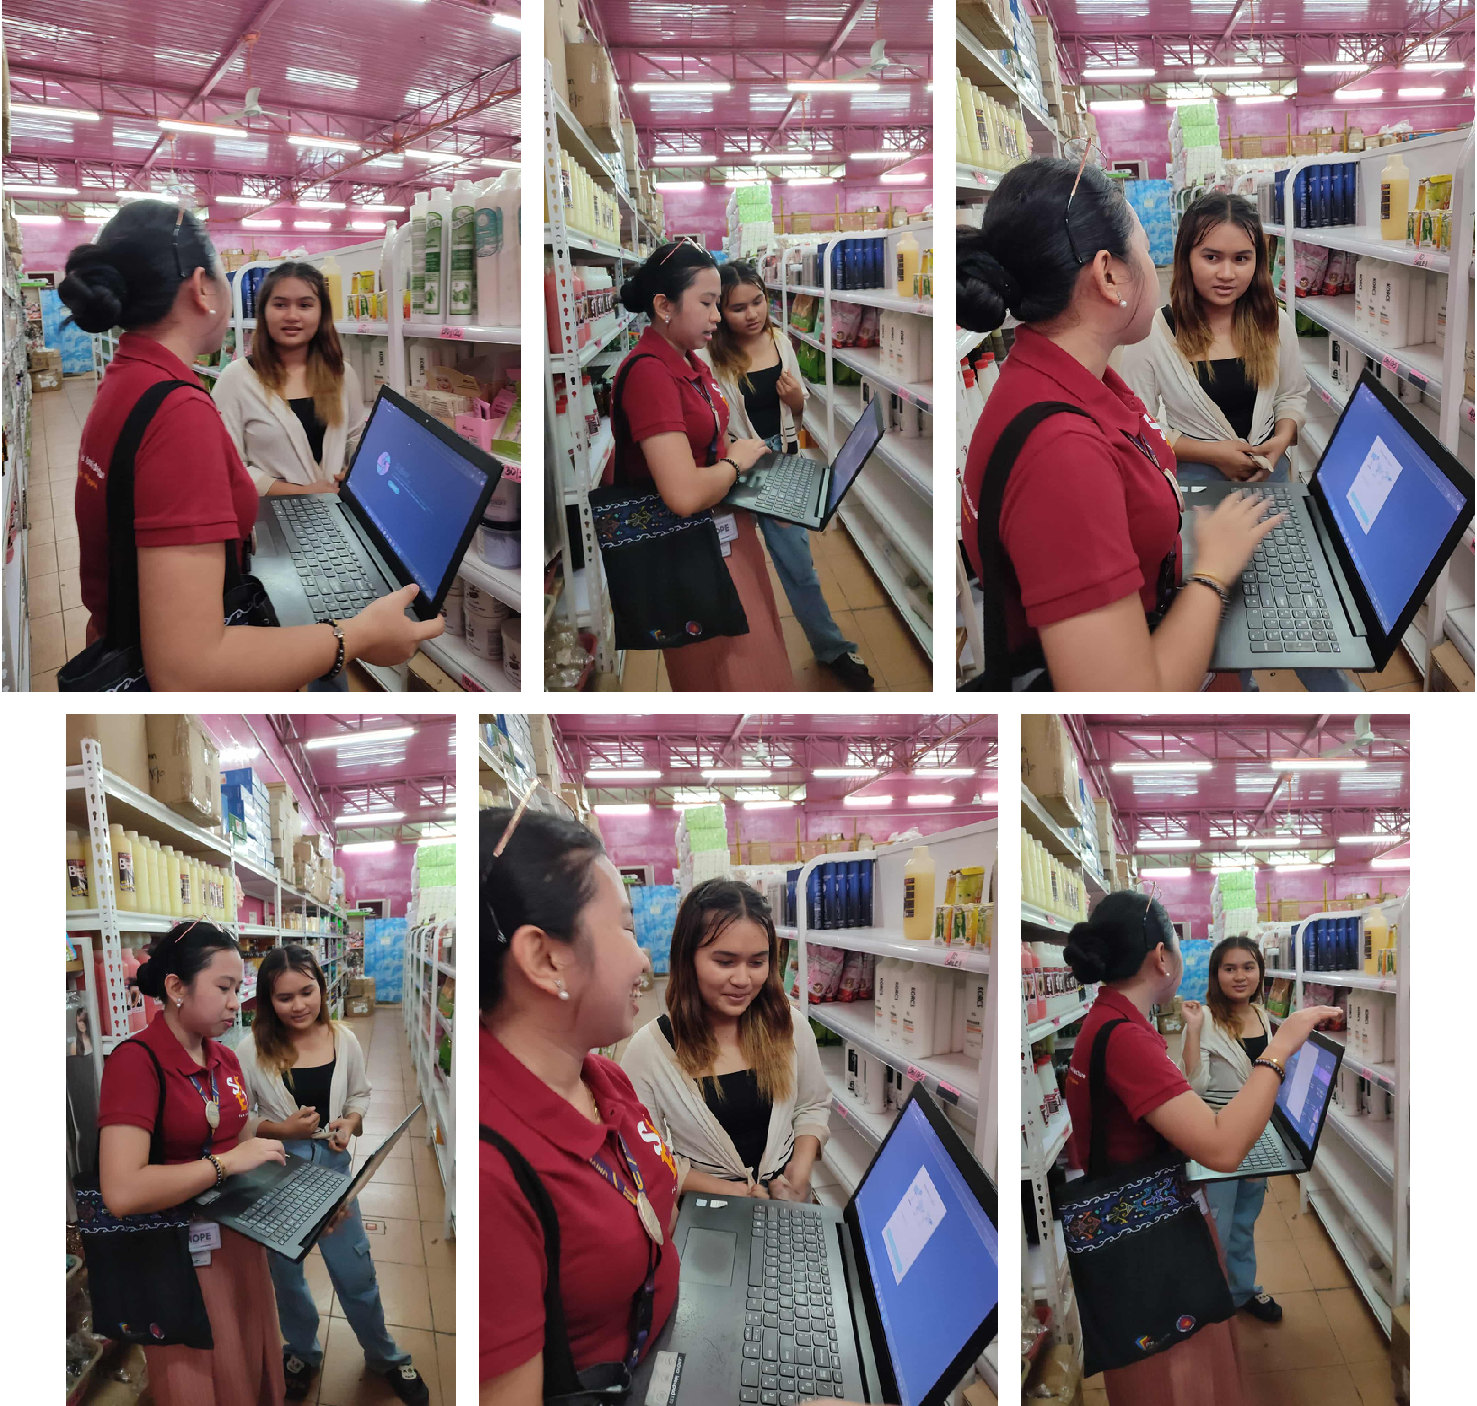
\includegraphics[width=1\textwidth]{app/H.pdf}
\end{center}

\clearpage

\begin{center}
	% Remove \thispagestyle{plain} to maintain consistent page numbering
	{\bf APPENDIX I}\\[24pt]
\end{center}
\addcontentsline{toc}{section}{APPENDIX I}

\begin{center}
	FUNCTIONAL AND USABILITY TESTING CONDUCTED
\end{center}

\begin{center}
	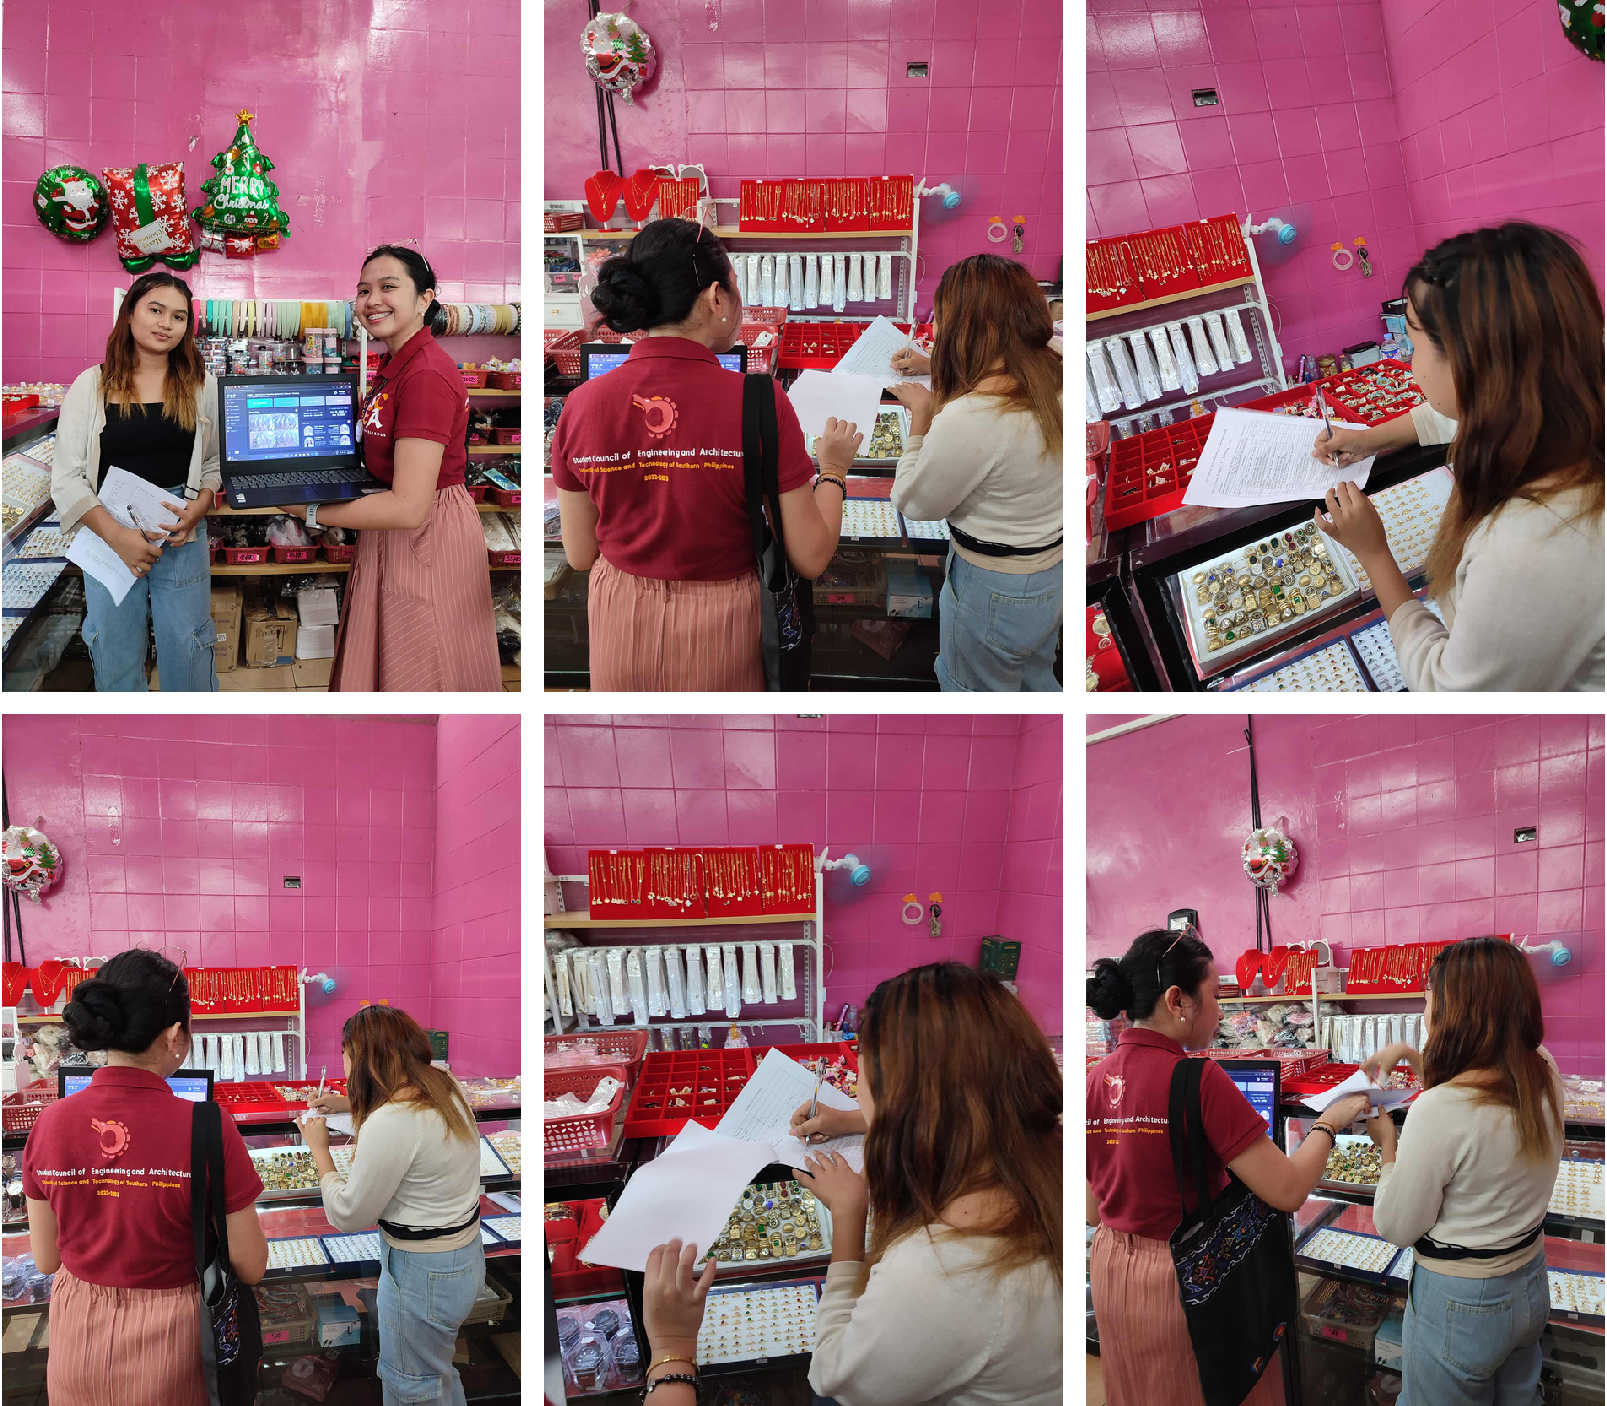
\includegraphics[width=1\textwidth]{app/I.pdf}
\end{center}

\clearpage

\begin{center}
	{\bf APPENDIX J}
\end{center}
\addcontentsline{toc}{section}{APPENDIX J}

\begin{center}
	NOMINATION OF MEMBERS FOR ORAL EXAMINATION PANEL FORM
\end{center}

\begin{center}
	
\includegraphics[width=1\textwidth]{app/L.pdf}
\end{center}

\clearpage

\begin{center}
	{\bf APPENDIX K}
\end{center}
\addcontentsline{toc}{section}{APPENDIX K}

\begin{center}
	APPROVED APPLICATION FOR ORAL DEFENSE FORMS
\end{center}

\begin{center}
	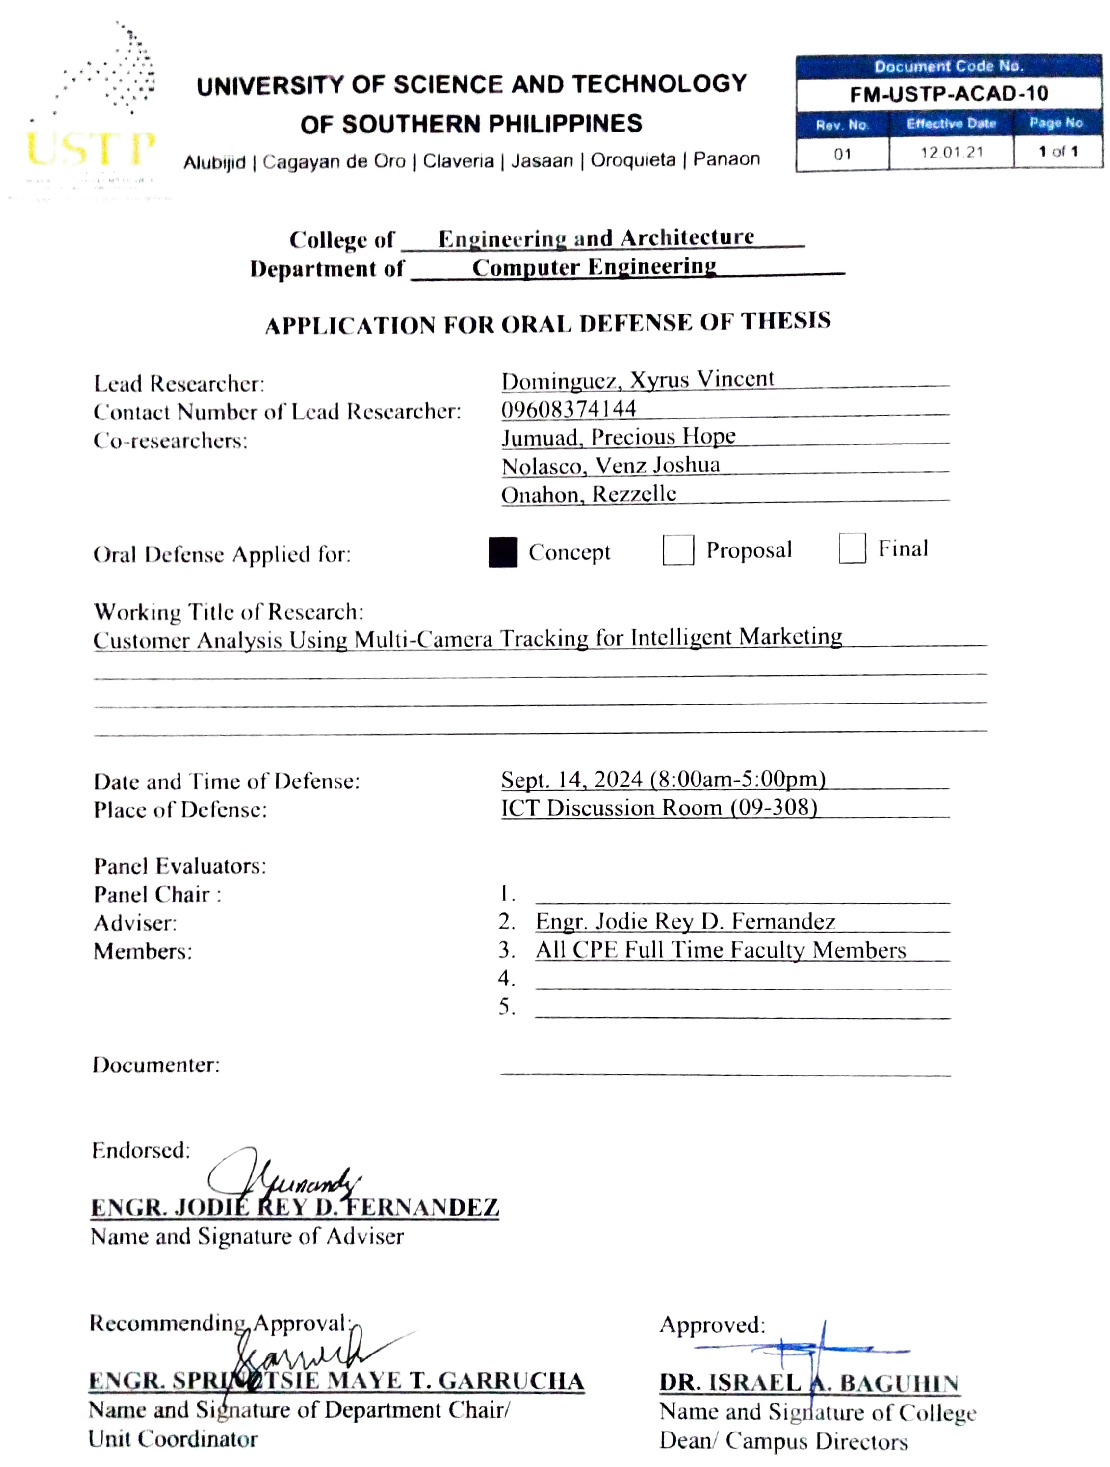
\includegraphics[width=0.9\textwidth]{app/M.pdf}
	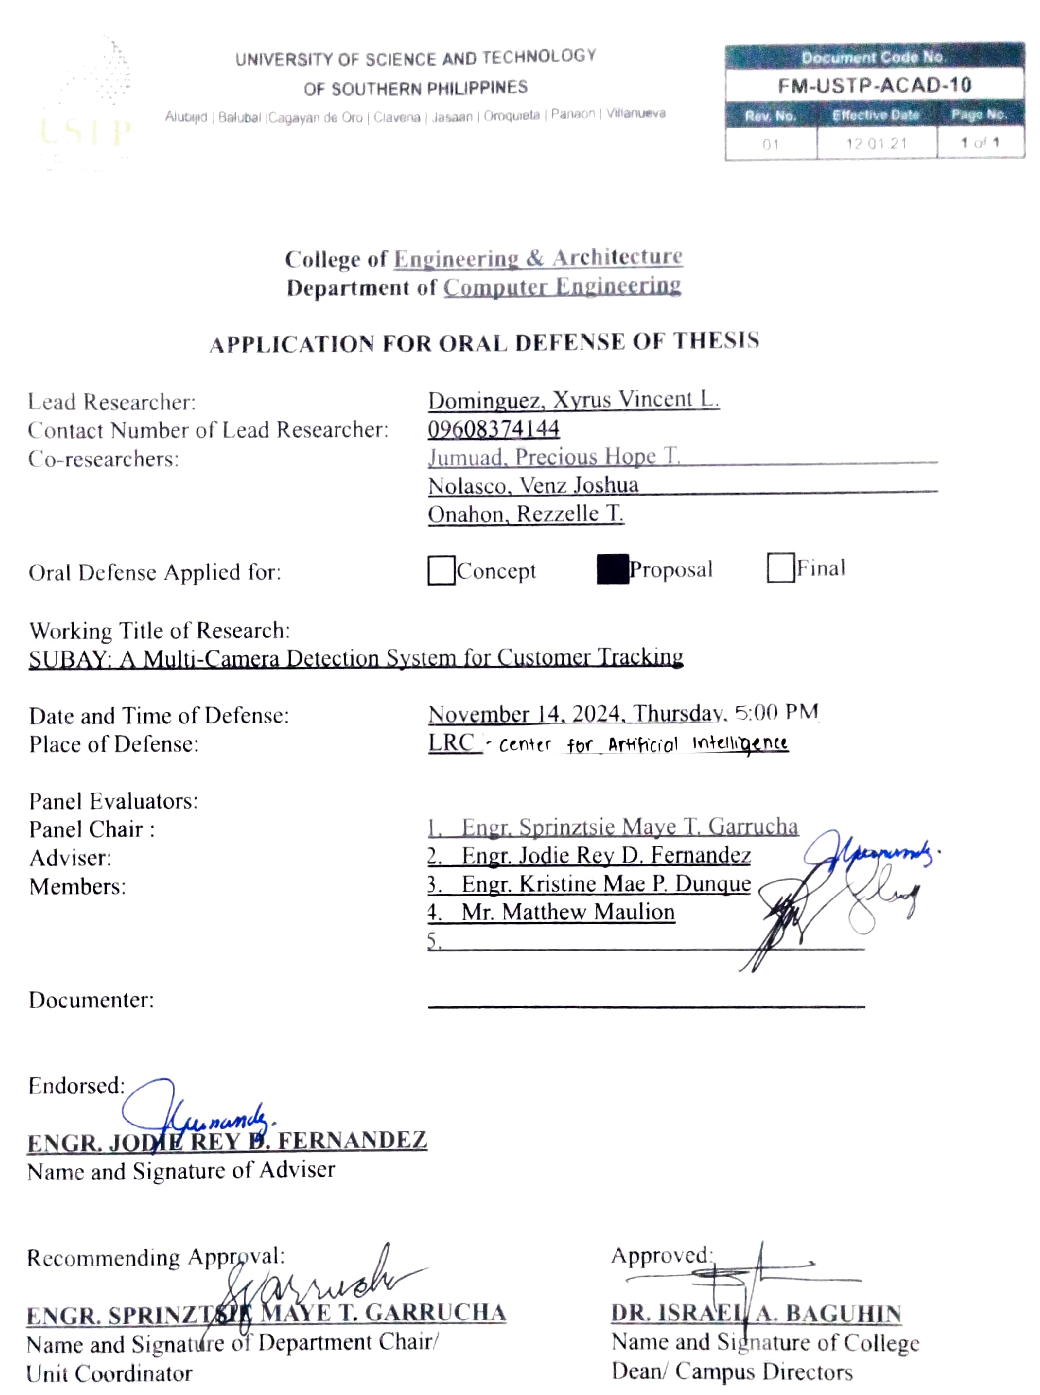
\includegraphics[width=0.9\textwidth]{app/N.pdf}
	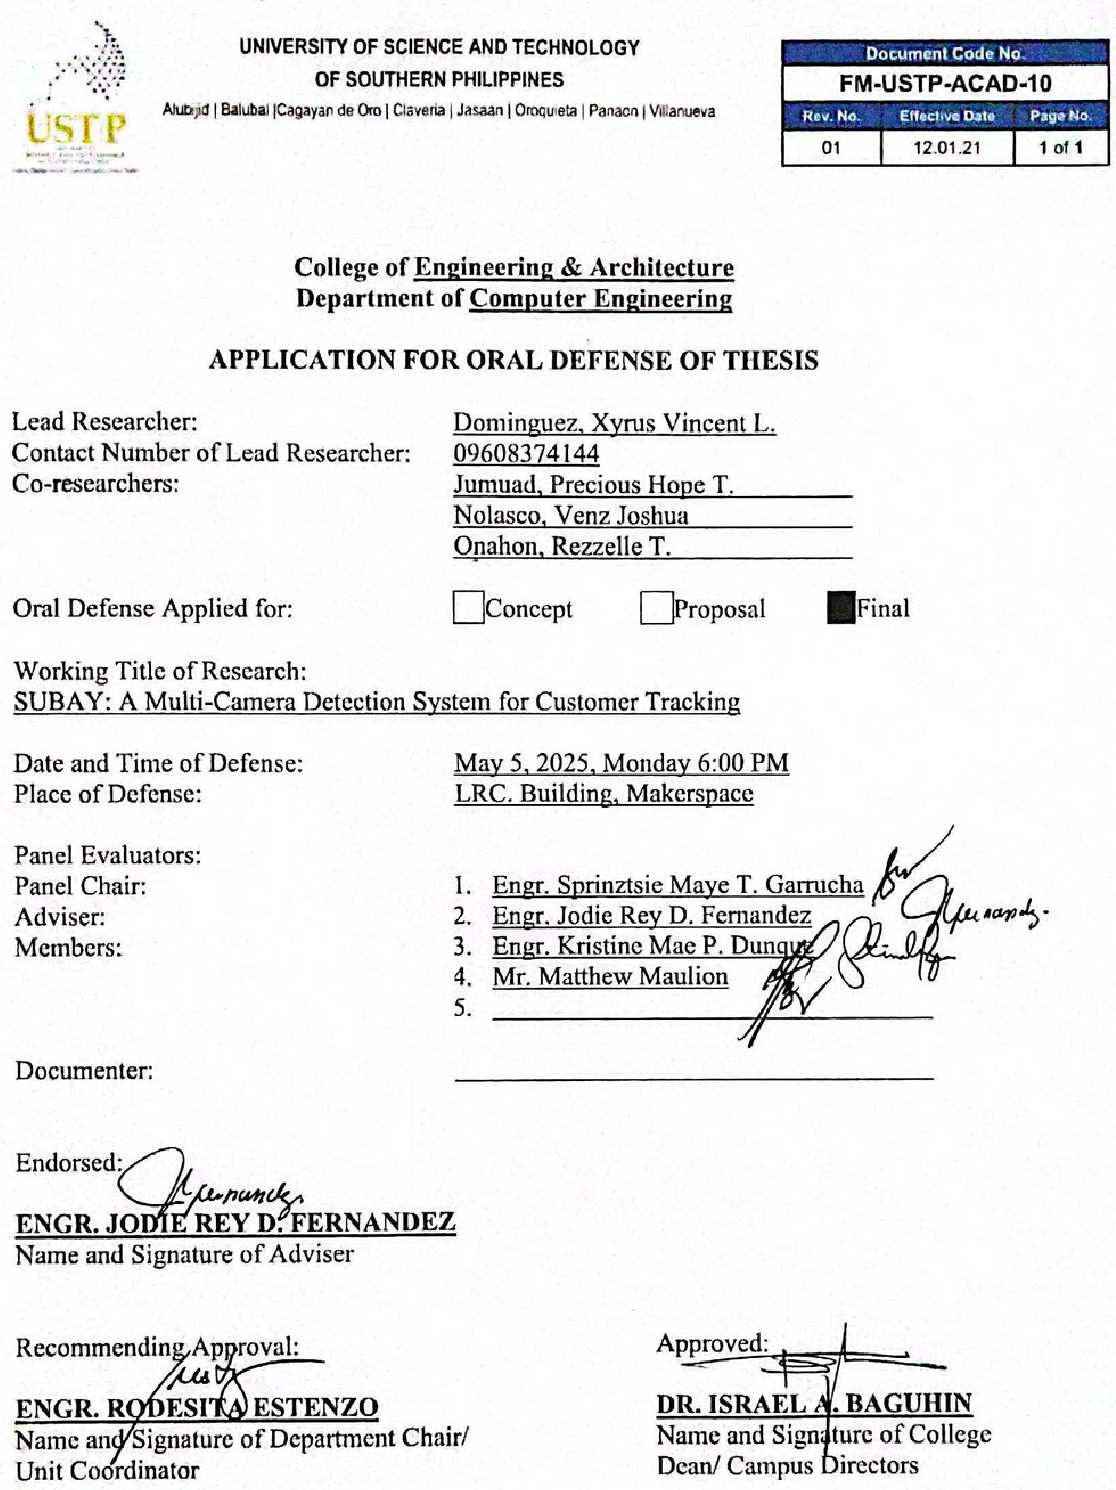
\includegraphics[width=0.9\textwidth]{app/O.pdf}
\end{center}

\clearpage

\begin{center}
	{\bf APPENDIX L}
\end{center}
\addcontentsline{toc}{section}{APPENDIX L}

\begin{center}
	REVISION MATRIX
\end{center}

\begin{center}
	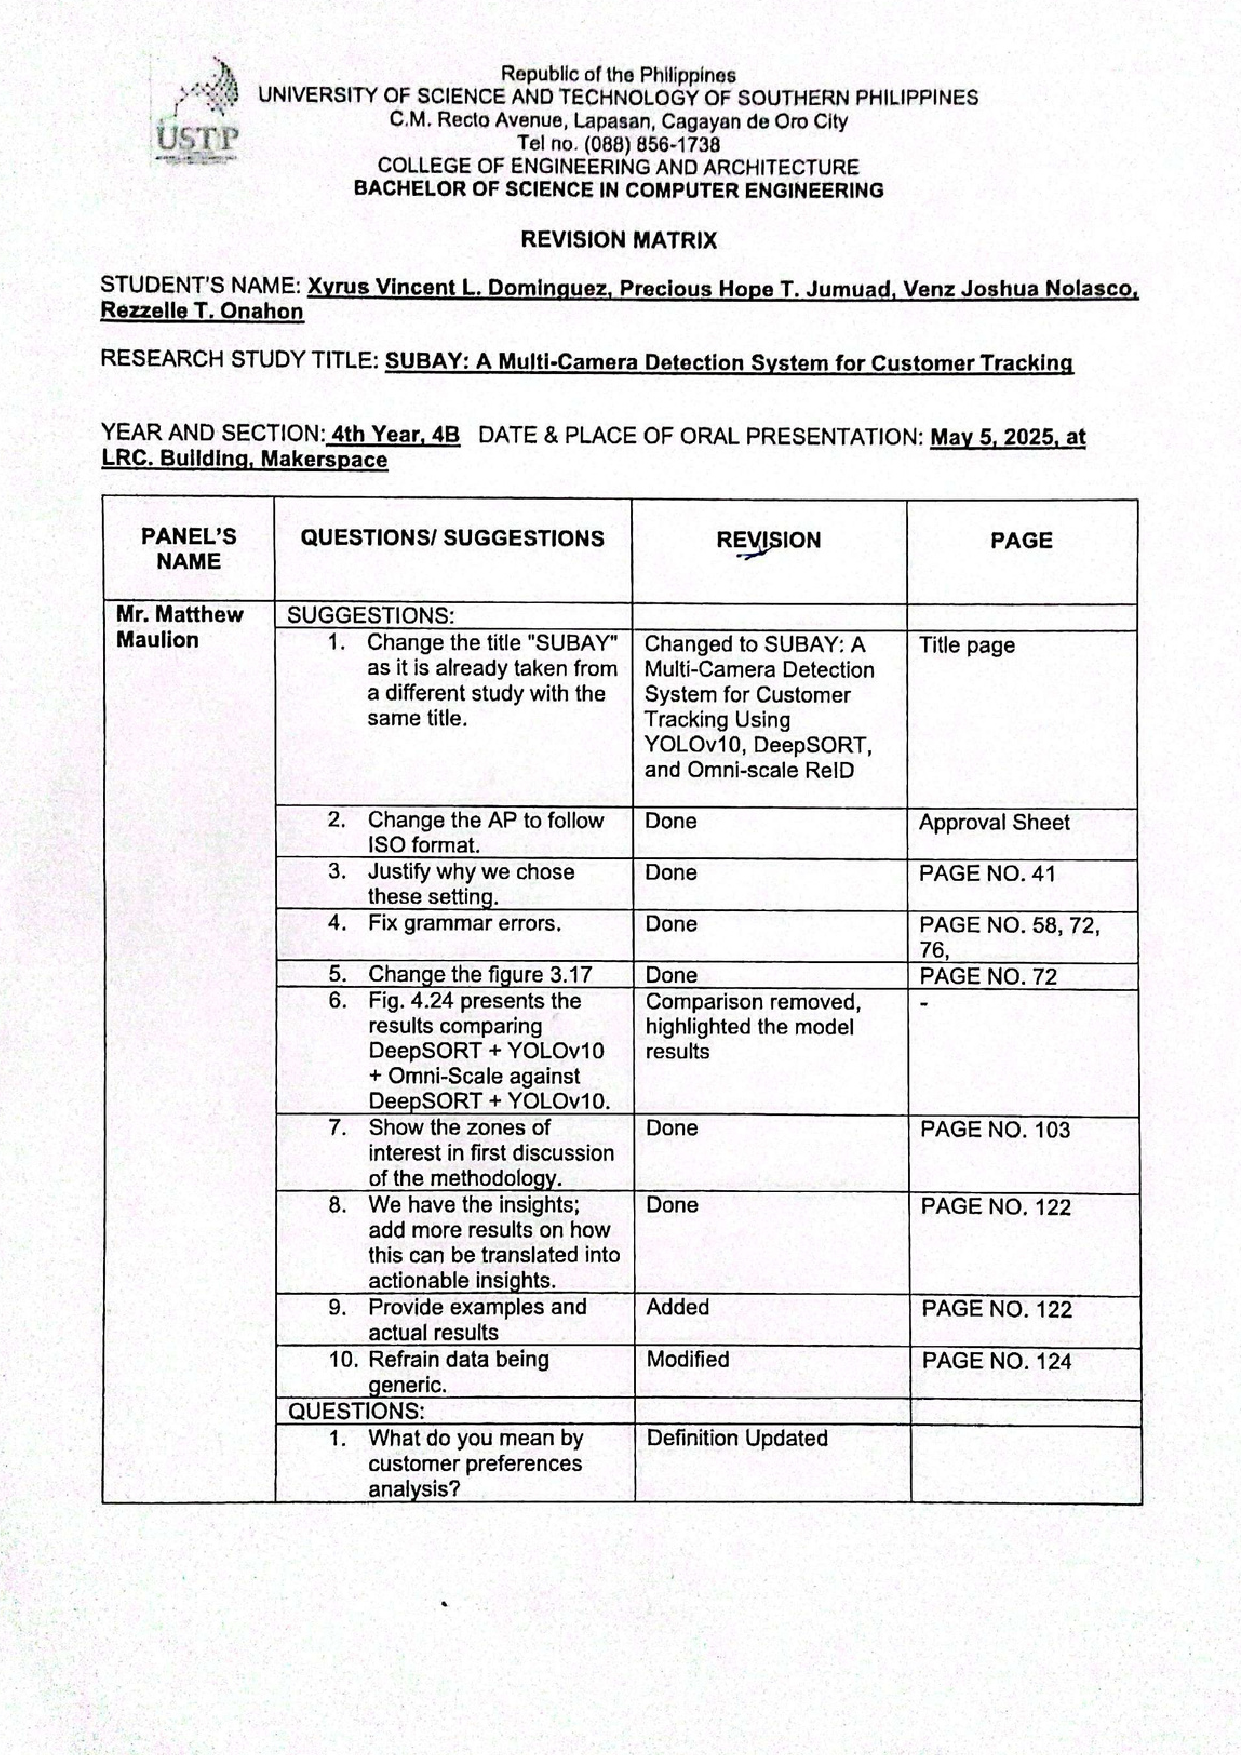
\includegraphics[width=0.93\textwidth]{app/L1.pdf}
	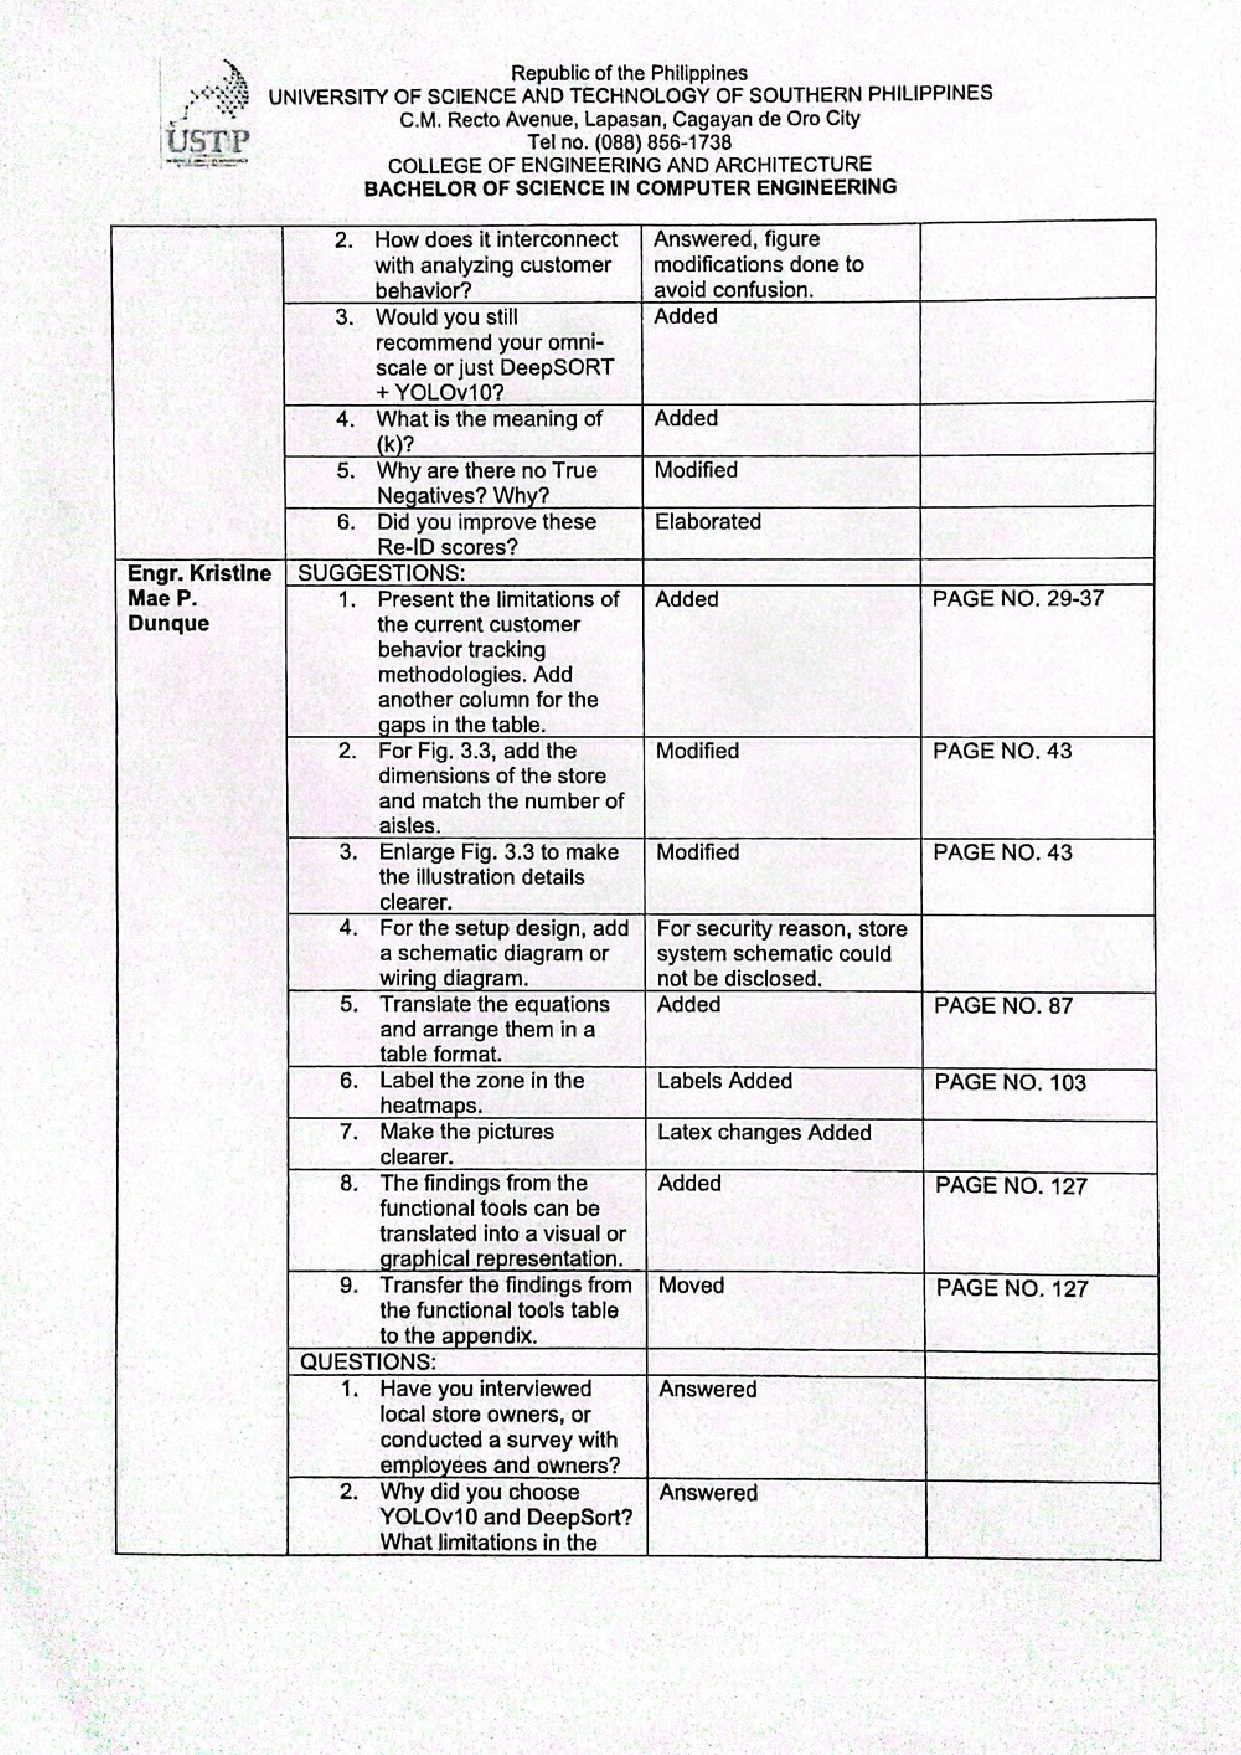
\includegraphics[width=1\textwidth]{app/L2.pdf}
	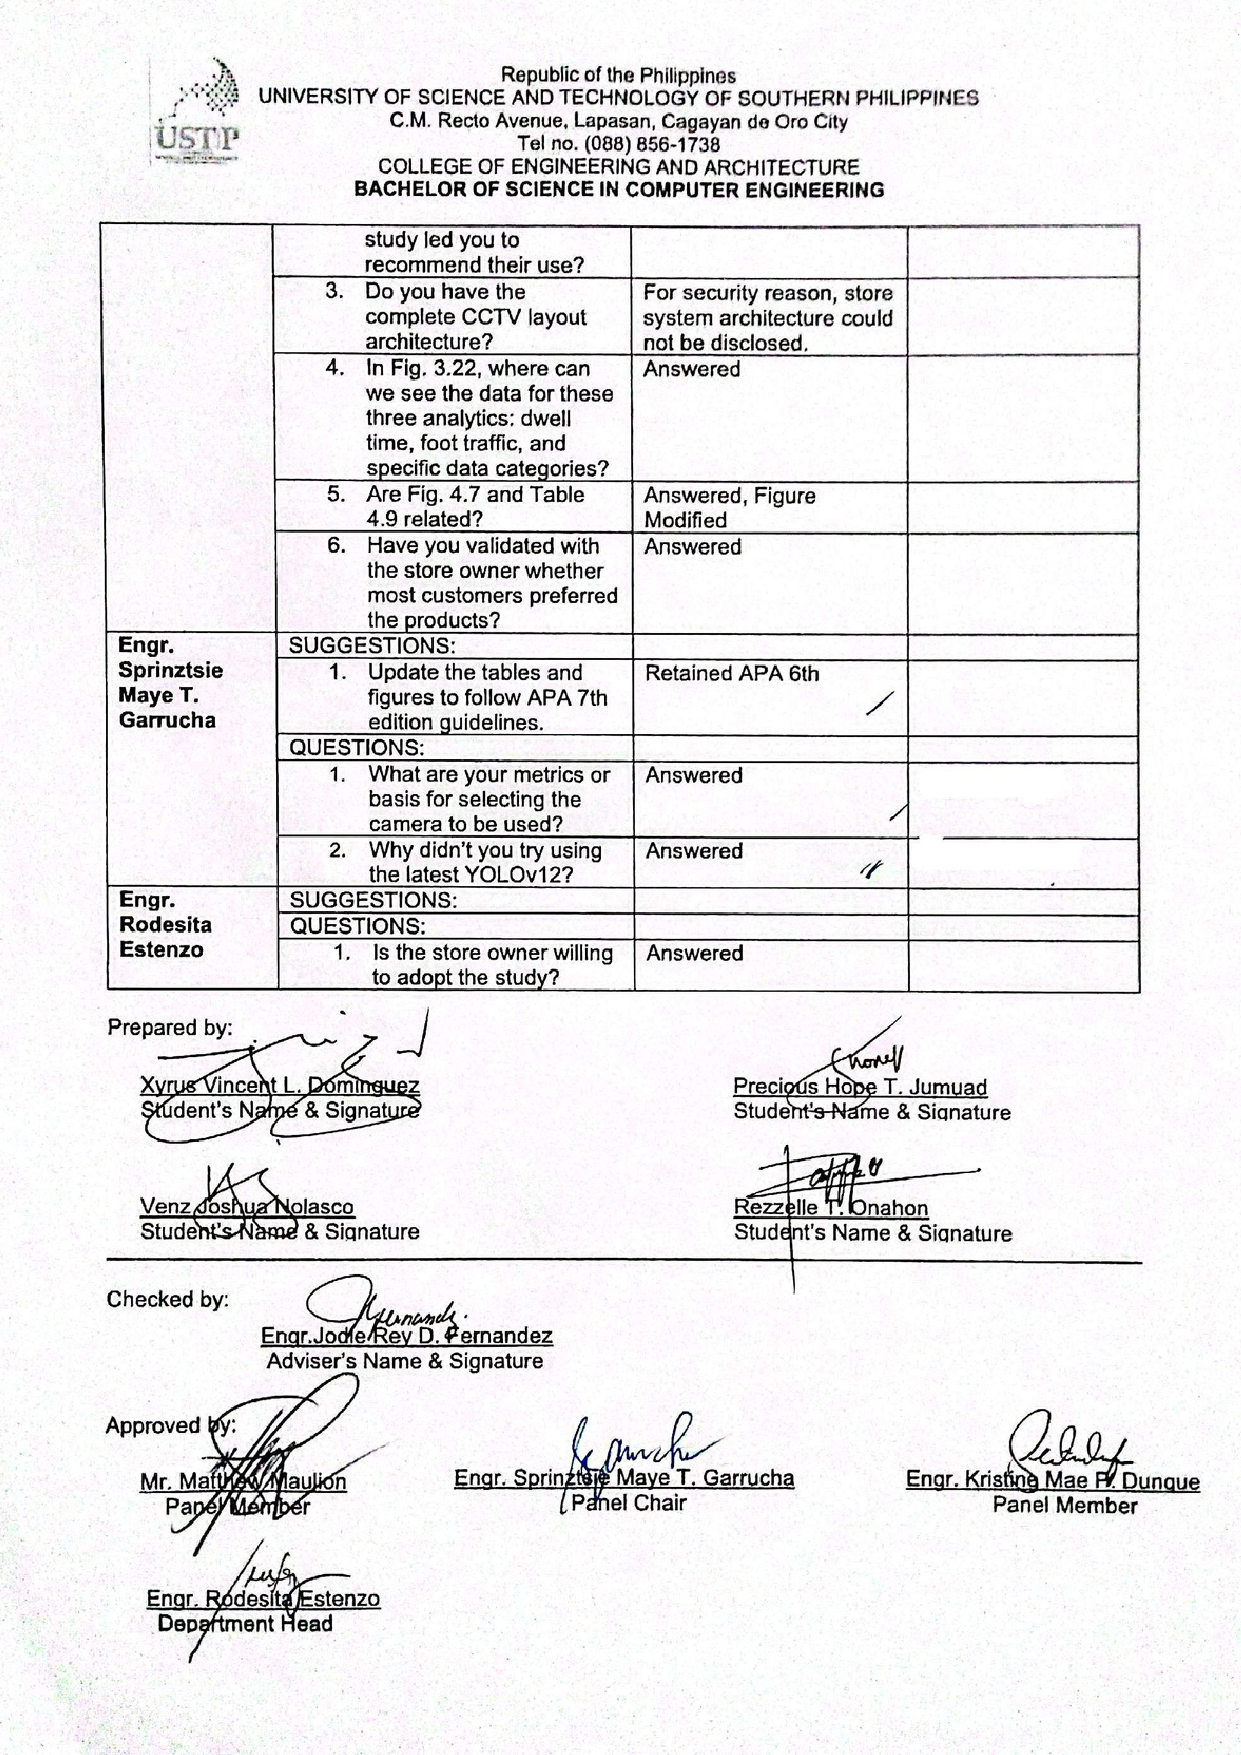
\includegraphics[width=1\textwidth]{app/L3.pdf}
\end{center}

\clearpage

\begin{center}
	% Remove \thispagestyle{plain} to maintain consistent page numbering
	{\bf APPENDIX M}\\[24pt]
\end{center}
\addcontentsline{toc}{section}{APPENDIX M}

\begin{center}
	THESIS PLAGIARISM CHECKER RESULT
\end{center}

\begin{center}
	\centering
	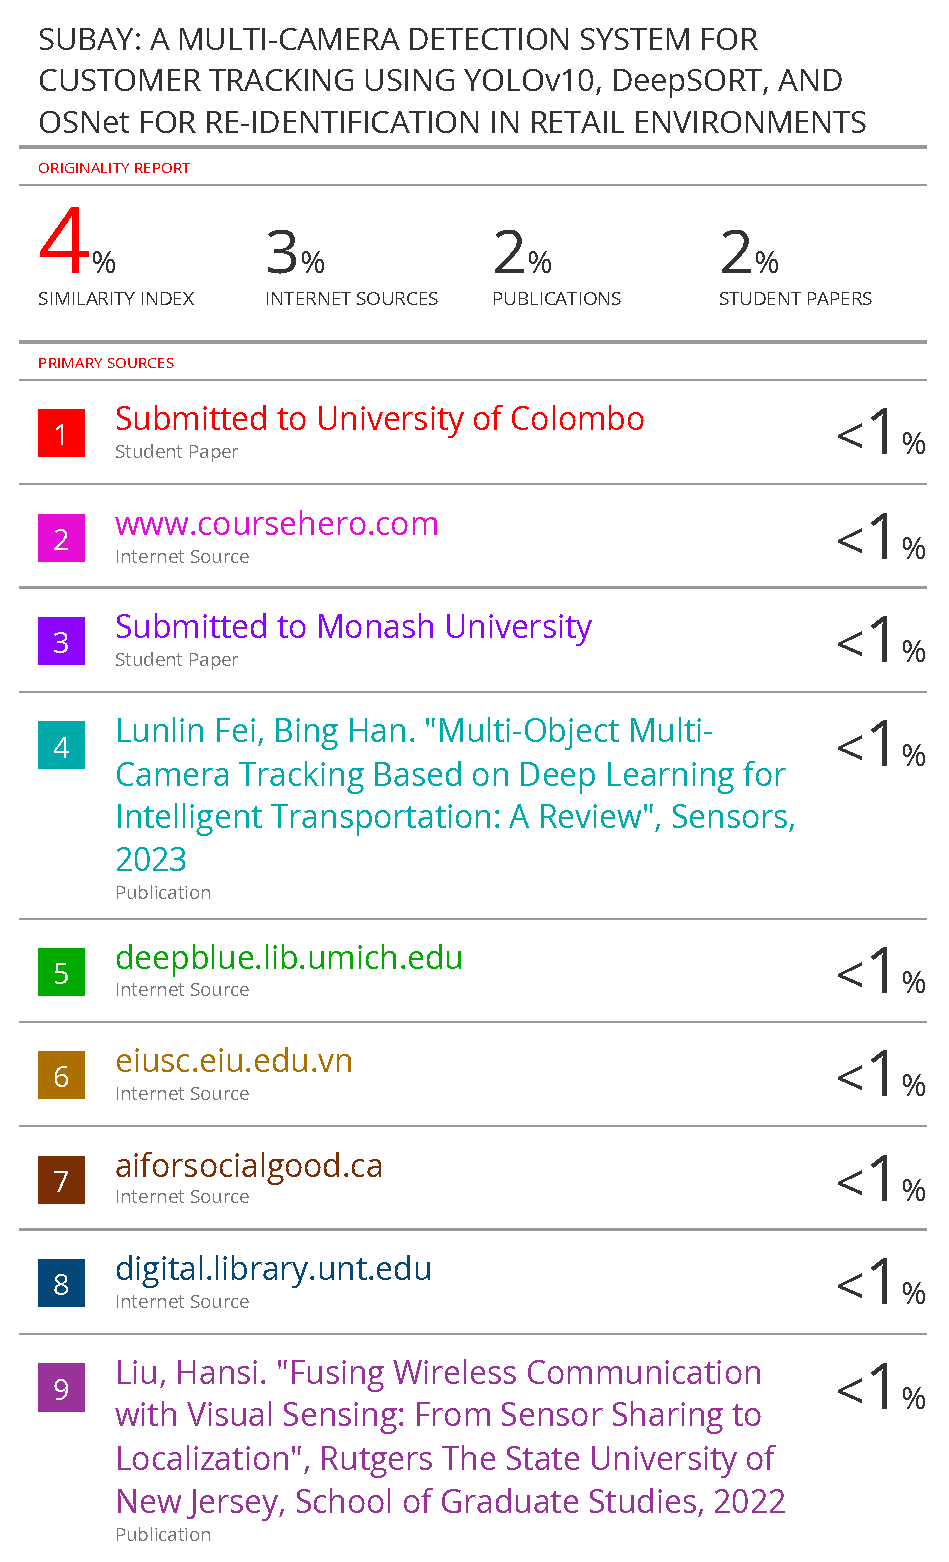
\includegraphics[width=0.75\textwidth]{app/J1.pdf}
	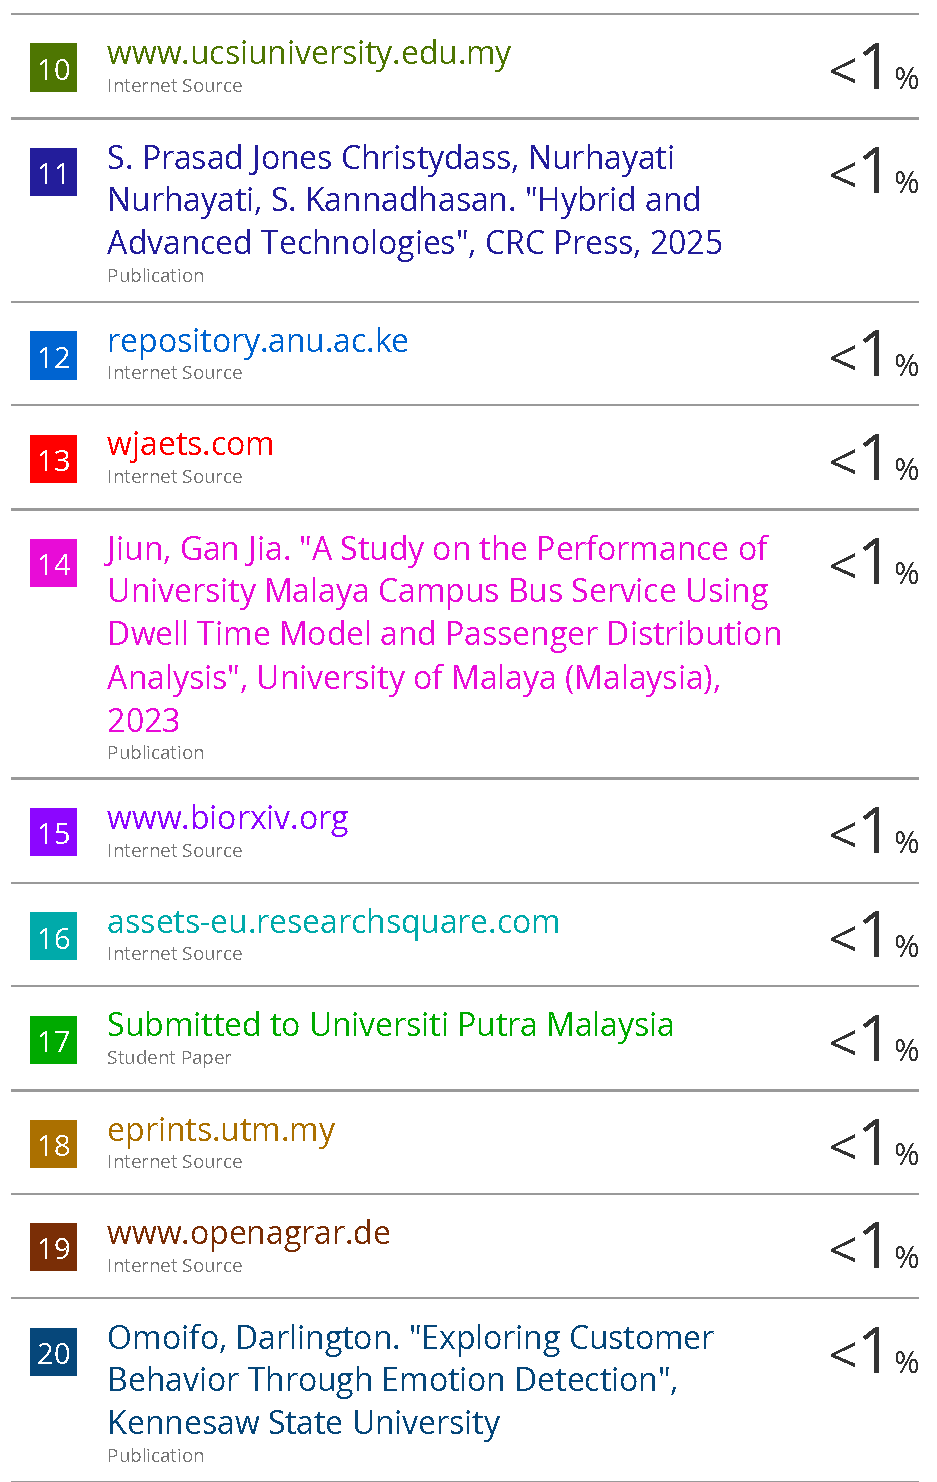
\includegraphics[width=0.75\textwidth]{app/J2.pdf}
	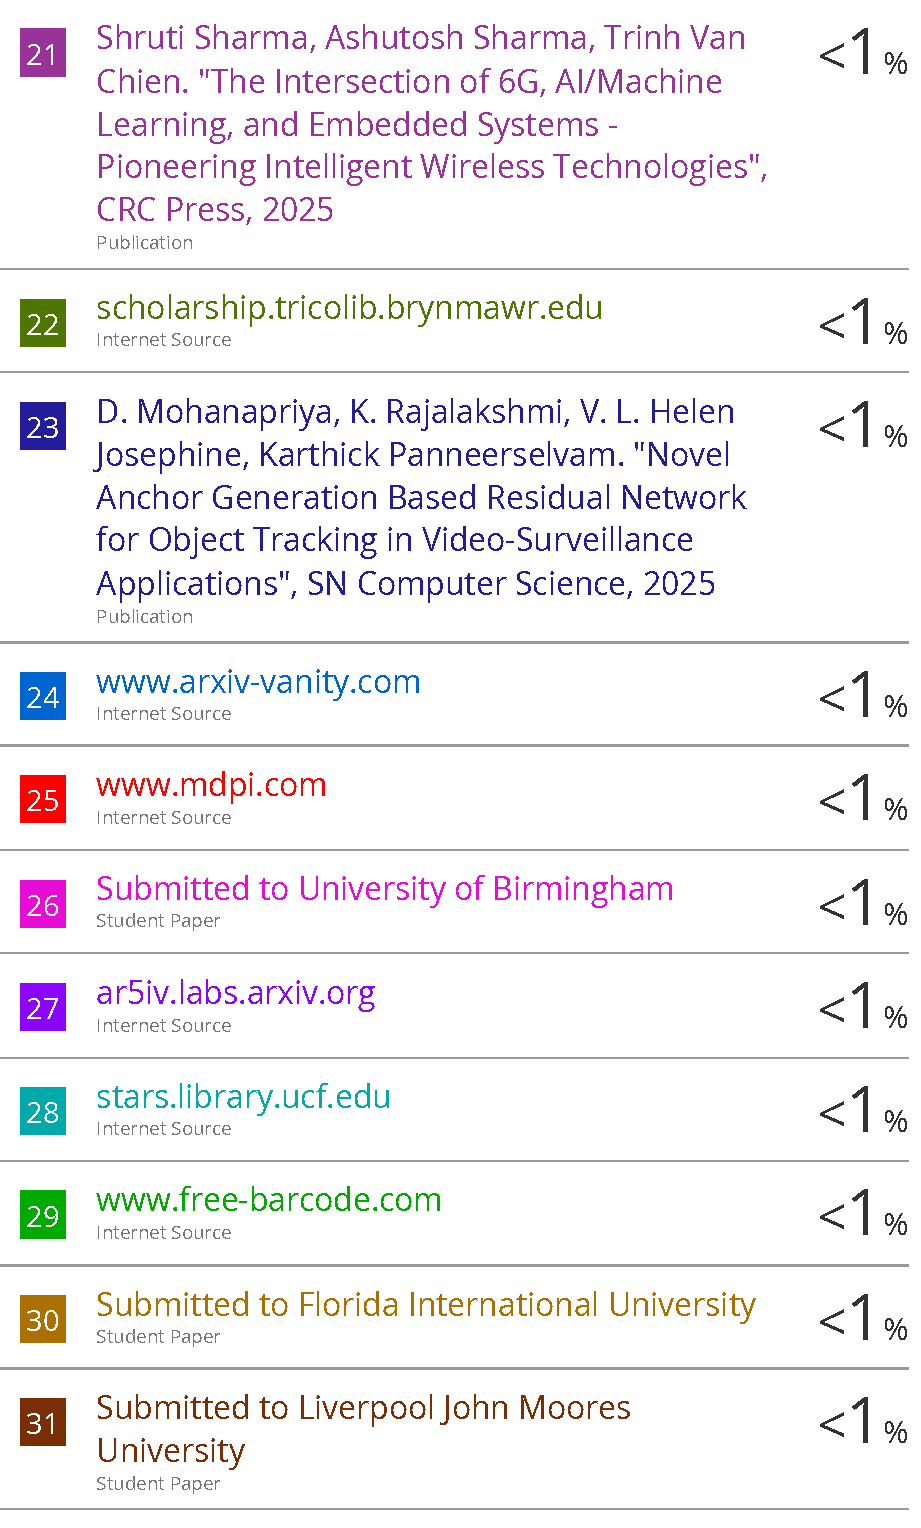
\includegraphics[width=0.75\textwidth]{app/J3.pdf}
	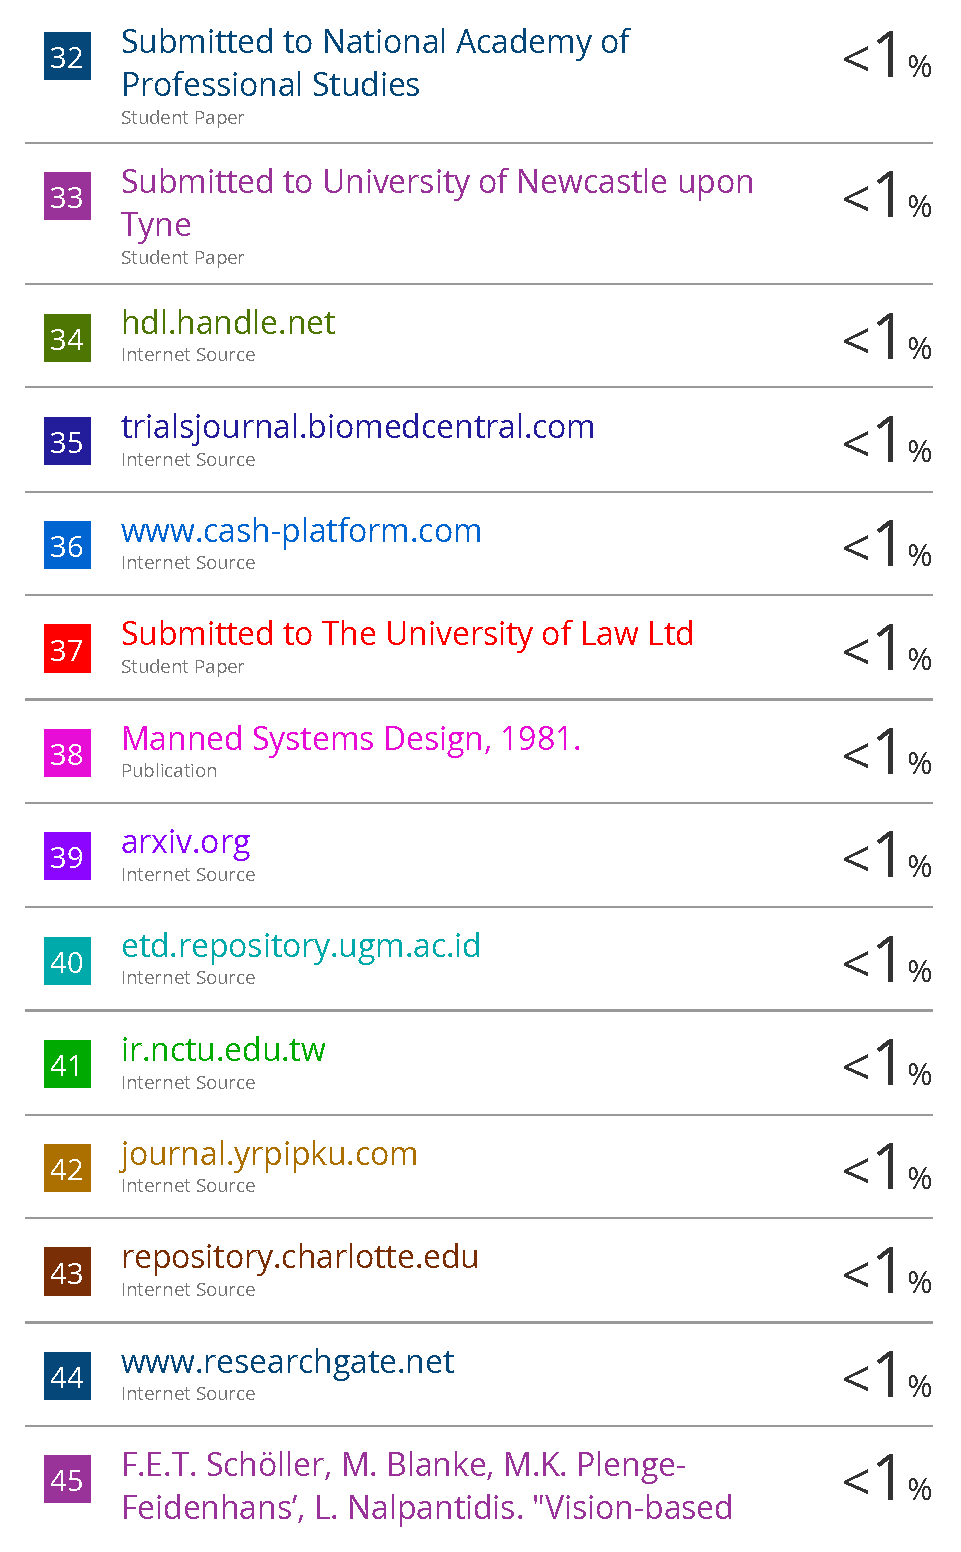
\includegraphics[width=0.75\textwidth]{app/J4.pdf}
	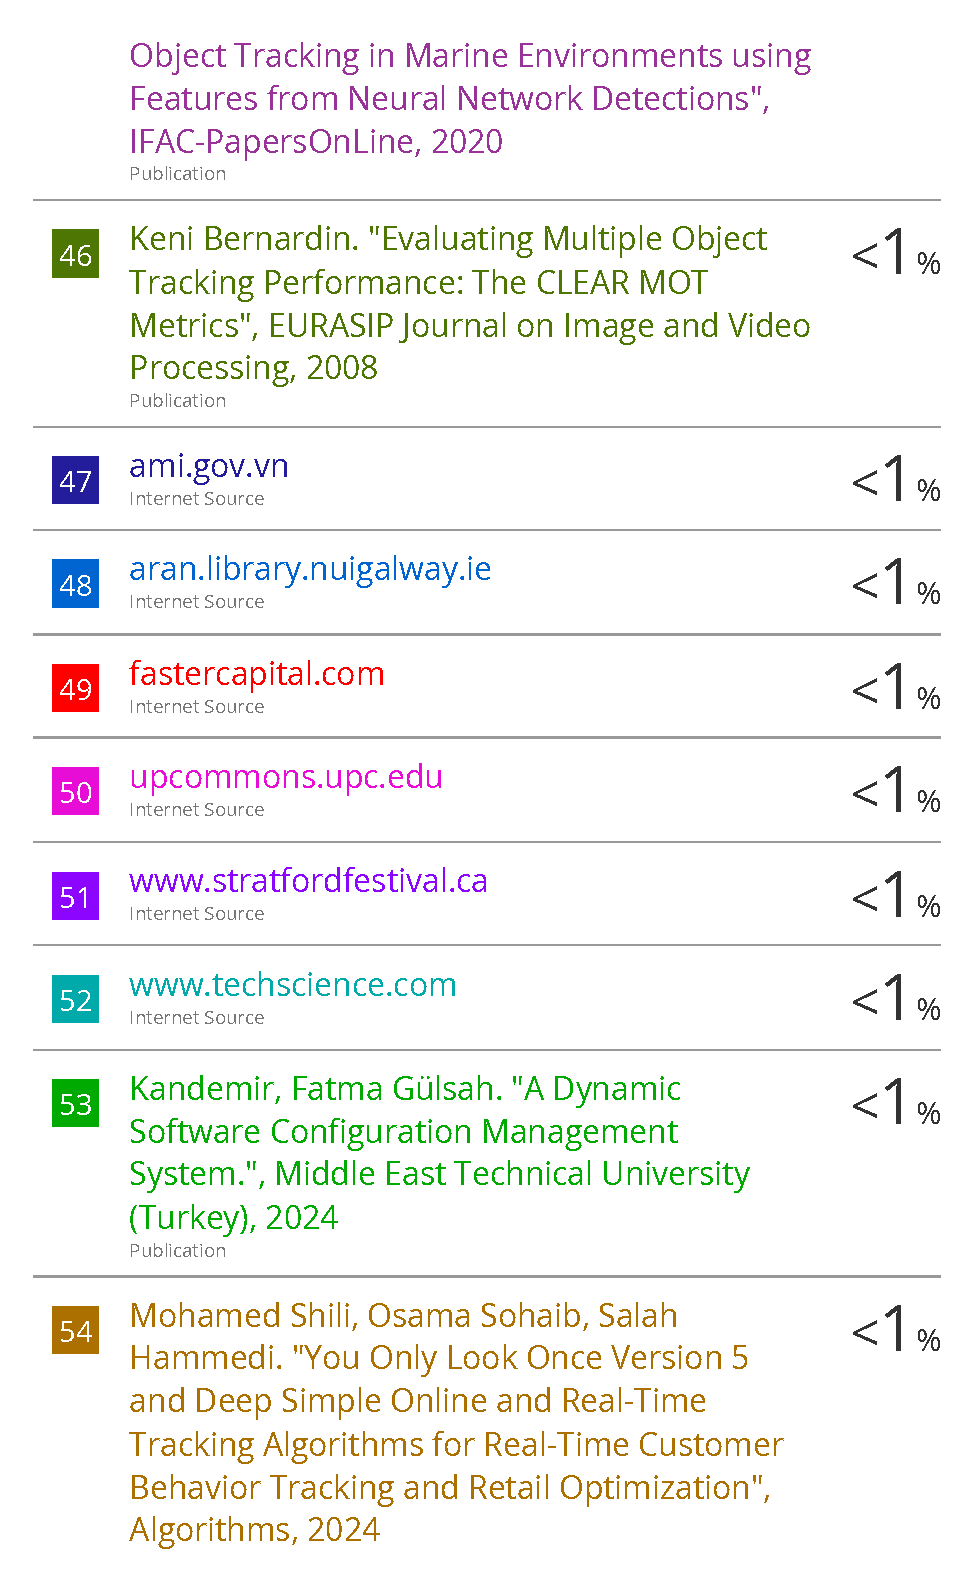
\includegraphics[width=0.75\textwidth]{app/J5.pdf}
	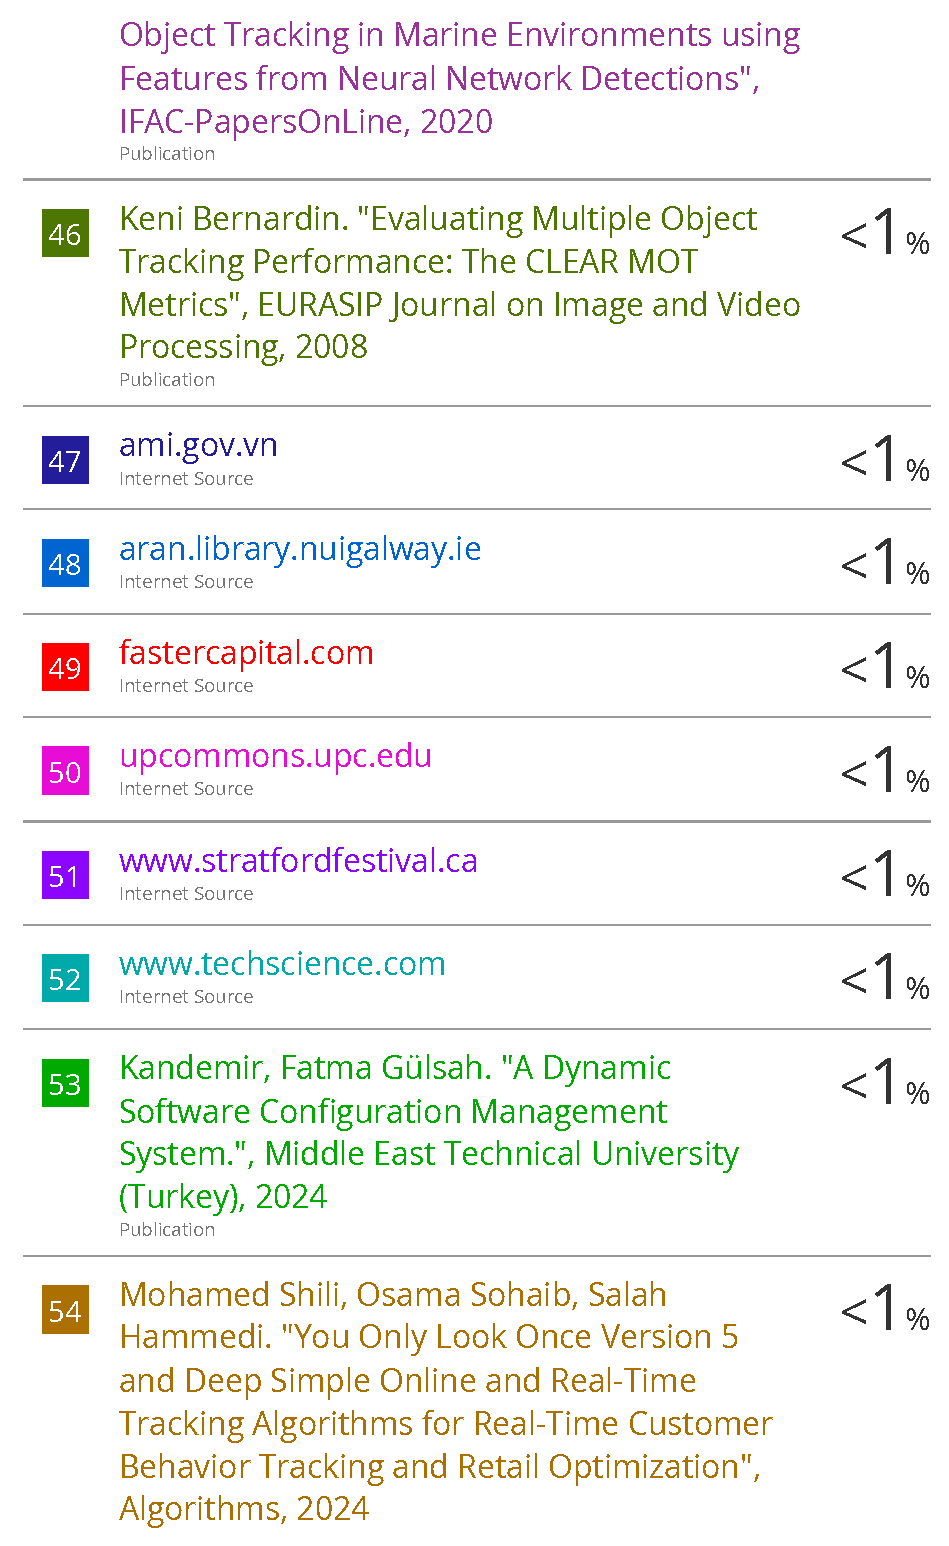
\includegraphics[width=0.75\textwidth]{app/J6.pdf}
\end{center}

\clearpage

\begin{center}
	{\bf APPENDIX N}
\end{center}
\addcontentsline{toc}{section}{APPENDIX N}

\begin{center}
	PROOFREADING CERTIFICATE AND REPORT OF RATING
\end{center}

\begin{center}
	
\includegraphics[width=1\textwidth]{app/K1.pdf}
	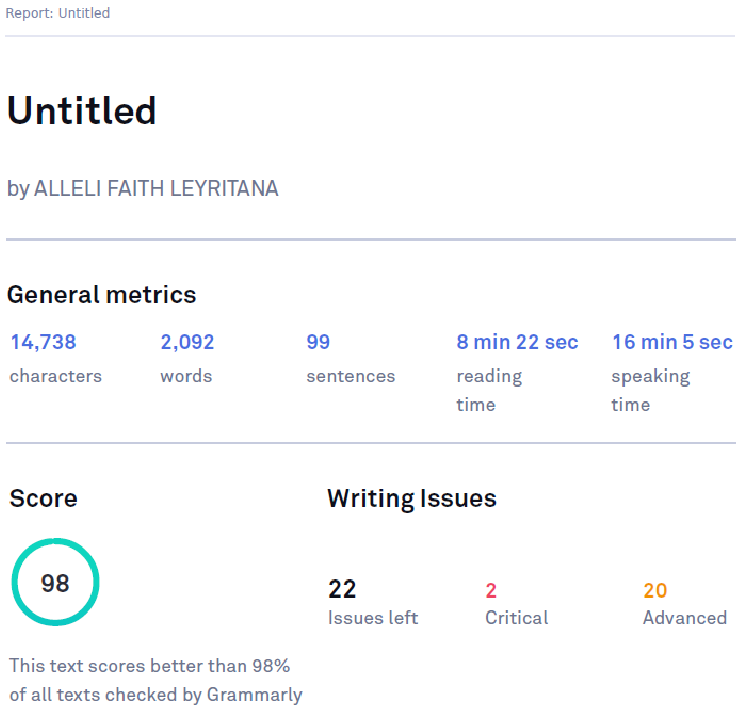
\includegraphics[width=\textwidth]{app/K2.pdf}
\end{center}

\clearpage